% Options for packages loaded elsewhere
\PassOptionsToPackage{unicode}{hyperref}
\PassOptionsToPackage{hyphens}{url}
%
\documentclass[
]{article}
\usepackage{amsmath,amssymb}
\usepackage{iftex}
\ifPDFTeX
  \usepackage[T1]{fontenc}
  \usepackage[utf8]{inputenc}
  \usepackage{textcomp} % provide euro and other symbols
\else % if luatex or xetex
  \usepackage{unicode-math} % this also loads fontspec
  \defaultfontfeatures{Scale=MatchLowercase}
  \defaultfontfeatures[\rmfamily]{Ligatures=TeX,Scale=1}
\fi
\usepackage{lmodern}
\ifPDFTeX\else
  % xetex/luatex font selection
\fi
% Use upquote if available, for straight quotes in verbatim environments
\IfFileExists{upquote.sty}{\usepackage{upquote}}{}
\IfFileExists{microtype.sty}{% use microtype if available
  \usepackage[]{microtype}
  \UseMicrotypeSet[protrusion]{basicmath} % disable protrusion for tt fonts
}{}
\makeatletter
\@ifundefined{KOMAClassName}{% if non-KOMA class
  \IfFileExists{parskip.sty}{%
    \usepackage{parskip}
  }{% else
    \setlength{\parindent}{0pt}
    \setlength{\parskip}{6pt plus 2pt minus 1pt}}
}{% if KOMA class
  \KOMAoptions{parskip=half}}
\makeatother
\usepackage{xcolor}
\usepackage[margin=1in]{geometry}
\usepackage{color}
\usepackage{fancyvrb}
\newcommand{\VerbBar}{|}
\newcommand{\VERB}{\Verb[commandchars=\\\{\}]}
\DefineVerbatimEnvironment{Highlighting}{Verbatim}{commandchars=\\\{\}}
% Add ',fontsize=\small' for more characters per line
\usepackage{framed}
\definecolor{shadecolor}{RGB}{248,248,248}
\newenvironment{Shaded}{\begin{snugshade}}{\end{snugshade}}
\newcommand{\AlertTok}[1]{\textcolor[rgb]{0.94,0.16,0.16}{#1}}
\newcommand{\AnnotationTok}[1]{\textcolor[rgb]{0.56,0.35,0.01}{\textbf{\textit{#1}}}}
\newcommand{\AttributeTok}[1]{\textcolor[rgb]{0.13,0.29,0.53}{#1}}
\newcommand{\BaseNTok}[1]{\textcolor[rgb]{0.00,0.00,0.81}{#1}}
\newcommand{\BuiltInTok}[1]{#1}
\newcommand{\CharTok}[1]{\textcolor[rgb]{0.31,0.60,0.02}{#1}}
\newcommand{\CommentTok}[1]{\textcolor[rgb]{0.56,0.35,0.01}{\textit{#1}}}
\newcommand{\CommentVarTok}[1]{\textcolor[rgb]{0.56,0.35,0.01}{\textbf{\textit{#1}}}}
\newcommand{\ConstantTok}[1]{\textcolor[rgb]{0.56,0.35,0.01}{#1}}
\newcommand{\ControlFlowTok}[1]{\textcolor[rgb]{0.13,0.29,0.53}{\textbf{#1}}}
\newcommand{\DataTypeTok}[1]{\textcolor[rgb]{0.13,0.29,0.53}{#1}}
\newcommand{\DecValTok}[1]{\textcolor[rgb]{0.00,0.00,0.81}{#1}}
\newcommand{\DocumentationTok}[1]{\textcolor[rgb]{0.56,0.35,0.01}{\textbf{\textit{#1}}}}
\newcommand{\ErrorTok}[1]{\textcolor[rgb]{0.64,0.00,0.00}{\textbf{#1}}}
\newcommand{\ExtensionTok}[1]{#1}
\newcommand{\FloatTok}[1]{\textcolor[rgb]{0.00,0.00,0.81}{#1}}
\newcommand{\FunctionTok}[1]{\textcolor[rgb]{0.13,0.29,0.53}{\textbf{#1}}}
\newcommand{\ImportTok}[1]{#1}
\newcommand{\InformationTok}[1]{\textcolor[rgb]{0.56,0.35,0.01}{\textbf{\textit{#1}}}}
\newcommand{\KeywordTok}[1]{\textcolor[rgb]{0.13,0.29,0.53}{\textbf{#1}}}
\newcommand{\NormalTok}[1]{#1}
\newcommand{\OperatorTok}[1]{\textcolor[rgb]{0.81,0.36,0.00}{\textbf{#1}}}
\newcommand{\OtherTok}[1]{\textcolor[rgb]{0.56,0.35,0.01}{#1}}
\newcommand{\PreprocessorTok}[1]{\textcolor[rgb]{0.56,0.35,0.01}{\textit{#1}}}
\newcommand{\RegionMarkerTok}[1]{#1}
\newcommand{\SpecialCharTok}[1]{\textcolor[rgb]{0.81,0.36,0.00}{\textbf{#1}}}
\newcommand{\SpecialStringTok}[1]{\textcolor[rgb]{0.31,0.60,0.02}{#1}}
\newcommand{\StringTok}[1]{\textcolor[rgb]{0.31,0.60,0.02}{#1}}
\newcommand{\VariableTok}[1]{\textcolor[rgb]{0.00,0.00,0.00}{#1}}
\newcommand{\VerbatimStringTok}[1]{\textcolor[rgb]{0.31,0.60,0.02}{#1}}
\newcommand{\WarningTok}[1]{\textcolor[rgb]{0.56,0.35,0.01}{\textbf{\textit{#1}}}}
\usepackage{longtable,booktabs,array}
\usepackage{calc} % for calculating minipage widths
% Correct order of tables after \paragraph or \subparagraph
\usepackage{etoolbox}
\makeatletter
\patchcmd\longtable{\par}{\if@noskipsec\mbox{}\fi\par}{}{}
\makeatother
% Allow footnotes in longtable head/foot
\IfFileExists{footnotehyper.sty}{\usepackage{footnotehyper}}{\usepackage{footnote}}
\makesavenoteenv{longtable}
\usepackage{graphicx}
\makeatletter
\def\maxwidth{\ifdim\Gin@nat@width>\linewidth\linewidth\else\Gin@nat@width\fi}
\def\maxheight{\ifdim\Gin@nat@height>\textheight\textheight\else\Gin@nat@height\fi}
\makeatother
% Scale images if necessary, so that they will not overflow the page
% margins by default, and it is still possible to overwrite the defaults
% using explicit options in \includegraphics[width, height, ...]{}
\setkeys{Gin}{width=\maxwidth,height=\maxheight,keepaspectratio}
% Set default figure placement to htbp
\makeatletter
\def\fps@figure{htbp}
\makeatother
\setlength{\emergencystretch}{3em} % prevent overfull lines
\providecommand{\tightlist}{%
  \setlength{\itemsep}{0pt}\setlength{\parskip}{0pt}}
\setcounter{secnumdepth}{-\maxdimen} % remove section numbering
\usepackage{hyperref}
\usepackage{amsmath}
\usepackage{amssymb}
\usepackage{graphicx}
\usepackage{fontspec}
\setmainfont{Cambria}
\setsansfont{Franklin Gothic Demi Cond}
\setmonofont{Courier New}
\usepackage[margin=1in]{geometry}
\usepackage{titlesec}
\titleformat{\section}{\Huge\bfseries\color{black}}{\thesection}{1em}{}
\titleformat{\subsection}{\huge\bfseries\color{black}}{\thesubsection}{1em}{}
\titleformat{\subsubsection}{\LARGE\bfseries\color{black}}{\thesubsubsection}{1em}{}
\usepackage{tocloft}
\renewcommand{\cftsecfont}{\small}
\renewcommand{\cftsubsecfont}{\footnotesize}
\renewcommand{\cftsecpagefont}{\small}
\renewcommand{\cftsubsecpagefont}{\footnotesize}
\renewcommand{\cftsecleader}{\cftdotfill{\cftdotsep}}
\ifLuaTeX
  \usepackage{selnolig}  % disable illegal ligatures
\fi
\usepackage{bookmark}
\IfFileExists{xurl.sty}{\usepackage{xurl}}{} % add URL line breaks if available
\urlstyle{same}
\hypersetup{
  hidelinks,
  pdfcreator={LaTeX via pandoc}}

\author{}
\date{\vspace{-2.5em}}

\begin{document}

\begin{titlepage}
    \begin{center}
        \textbf{\LARGE RÉPUBLIQUE DU SÉNÉGAL}\\[0.1cm]
        
\includegraphics[width=3cm]{images/Logo1.jpg} \\[0.1cm]  % Insère le chemin de ton logo
        \textbf{\large Un Peuple - Un But - Une Foi}\\[0.2cm]
        
        \textbf{\LARGE Ministère de l'Économie, du Plan et de la Coopération}\\[0.1cm]
        
\includegraphics[width=4cm]{images/Logo2.png} \\[0.1cm] 
        
        \textbf{\large Agence Nationale de la Statistique et de la Démographie (ANSD)}\\[0.2cm]
        
        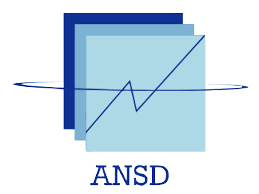
\includegraphics[width=4cm]{images/Logo3.png} \\[0.1cm]  
        
        \textbf{\large École Nationale de la Statistique et de l'Analyse Économique Pierre Ndiaye (ENSAE)}\\[0.4cm]
        
\includegraphics[width=3cm]{images/Logo4.png} \\[0.1cm]
        
        \textbf{\LARGE PROJET STATISTIQUES SOUS R }\\[0.3cm]
        \textbf{\Huge \color{blue} \textsf{TP10 : Traitement des questions ouvertes avec R : Text mining}}\\[0.2cm]
        \rule{\linewidth}{0.2mm} \\[0.5cm]
        
        \begin{minipage}{0.5\textwidth}
    \begin{flushleft} \large
        \emph{\textsf{Rédigé par :}}\\
        \textbf{Mame Balla BOUSSO}\\
        \textbf{Paul BALAFAI}\\
        \textit{Elèves ingénieurs statisticiens économistes}
    \end{flushleft}
\end{minipage}
        \hfill
        \begin{minipage}{0.4\textwidth}
            \begin{flushright} \large
                \emph{\textsf{Sous la supervision de :}} \\
                \textbf{M. Aboubacar HEMA}\\
                \textit{ANALYSTE DE RECHERCHE CHEZ IFPRI }
            \end{flushright}
        \end{minipage}

        \vfill

        {\large \textsf{Année scolaire : 2024/2025}}\\[0.5cm]
        
    \end{center}
\end{titlepage}

\newpage

\section{Sommaire}\label{sommaire}

\begin{itemize}
\tightlist
\item
  \hyperref[analyse-textuelle-reponses-enquete]{Traitement des questions
  ouvertes avec R}

  \begin{itemize}
  \tightlist
  \item
    \hyperref[importation-nettoyage-donnees]{1. Importation et Nettoyage
    des Données}
  \item
    \hyperref[exploration-pretraitement-textuel]{2. Exploration et
    Prétraitement Textuel}
  \item
    \hyperref[analyse-thematique-lda]{3. Analyse Thématique (LDA)}
  \item
    \hyperref[approche-alternative-bertopic]{4. Approche Alternative
    avec BERTopic}
  \item
    \hyperref[visualisation]{5. Catégorisation}
  \item
    \hyperref[conclusion]{CONCLUSION}
  \end{itemize}
\item
  \hyperref[references-webographiques]{Références}
\end{itemize}

\newpage

\section{INTRODUCTION}\label{sec:importation}

Le traitement automatique du langage naturel (TALN) regroupe un ensemble
de techniques permettant d'analyser, de comprendre et de transformer des
textes en données exploitables. Il existe plusieurs manières d'aborder
le traitement de texte, selon la nature des données et les objectifs
visés.

La forme la plus courante est l'analyse \textbf{supervisée}, où chaque
texte est associé à un label prédéfini. Ces labels peuvent par exemple
représenter des catégories binaires comme 0 ou 1, ou encore des
sentiments comme positif, négatif ou neutre. Dans ce contexte, on
entraîne un modèle à apprendre ces correspondances pour ensuite classer
de nouveaux textes.

Cependant, dans de nombreux cas, notamment dans les \textbf{questions
ouvertes d'enquêtes}, il n'existe aucune annotation préalable permettant
de guider l'apprentissage. Il devient alors nécessaire de structurer les
données ex nihilo, c'est-à-dire sans repère préalable, en regroupant les
textes selon leur \textbf{similarité sémantique}. C'est le domaine de
l'analyse \textbf{non supervisée}.

Dans ce cas, une solution consiste à effectuer une analyse thématique,
en divisant le corpus en un \textbf{nombre𝐾} de thèmes ou sujets, choisi
avec soin. Cette démarche vise à extraire les grandes lignes du contenu
textuel, en révélant les motifs récurrents présents dans les réponses.
Cela permet d'enrichir l'analyse qualitative des enquêtes, même en
l'absence de catégorisation préalable.

Dans cette étude, nous nous concentrerons spécifiquement sur cette
approche \textbf{non supervisée}. Nous mettrons en œuvre des techniques
disponibles dans le langage R, notamment grâce à des packages comme
\textbf{topicmodels (pour le modèle LDA)}, \textbf{tidytext}, et
\textbf{BERTopic} via le package \textbf{reticulate}, pour recourir à
des modèles sémantiques plus avancés.

\newpage

\section{1. Importation et Nettoyage des Données}\label{sec:importation}

\subsubsection{Chargement des packages}\label{chargement-des-packages}

\begin{Shaded}
\begin{Highlighting}[]
\FunctionTok{library}\NormalTok{(readxl)       }\CommentTok{\# Pour lire les fichiers Excel}
\FunctionTok{library}\NormalTok{(topicmodels)  }\CommentTok{\# Pour la modélisation thématique}
\FunctionTok{library}\NormalTok{(ggplot2)      }\CommentTok{\# Pour les visualisations}
\FunctionTok{library}\NormalTok{(dplyr)        }\CommentTok{\# Pour la manipulation de données}
\FunctionTok{library}\NormalTok{(tidytext)     }\CommentTok{\# Pour le traitement de texte}
\FunctionTok{library}\NormalTok{(tidyr)        }\CommentTok{\# Pour la gestion des données}
\FunctionTok{library}\NormalTok{(wordcloud)    }\CommentTok{\# Pour les nuages de mots}
\FunctionTok{library}\NormalTok{(tidyverse)    }\CommentTok{\# Collection de packages pour la science des données}
\FunctionTok{library}\NormalTok{(tm)           }\CommentTok{\# Pour le text mining}
\FunctionTok{library}\NormalTok{(SnowballC)    }\CommentTok{\# Pour le stemming}
\FunctionTok{library}\NormalTok{(stringr)      }\CommentTok{\# Pour la manipulation de strings}
\end{Highlighting}
\end{Shaded}

\subsection{Importation des données}\label{importation-des-donnuxe9es}

\begin{Shaded}
\begin{Highlighting}[]
\NormalTok{Enquête\_dopinion\_relative\_à\_la\_journée\_dintégration\_ }\OtherTok{\textless{}{-}} \FunctionTok{read\_excel}\NormalTok{(}\StringTok{"Data/Enquête\_dopinion\_relative\_à\_la\_journée\_dintégration).xlsx"}\NormalTok{)}
\NormalTok{Texte\_JI }\OtherTok{\textless{}{-}}\NormalTok{ Enquête\_dopinion\_relative\_à\_la\_journée\_dintégration\_}
\FunctionTok{head}\NormalTok{(Enquête\_dopinion\_relative\_à\_la\_journée\_dintégration\_)}
\end{Highlighting}
\end{Shaded}

\begin{verbatim}
## # A tibble: 6 x 4
##      id `Classe de l’étudiant :` `Nationalité de l'étudiant` Texte              
##   <dbl> <chr>                    <chr>                       <chr>              
## 1     1 AS2                      Congo                       <NA>               
## 2     2 ISEP1                    Cameroun                    Donner à temps le ~
## 3     3 AS2                      Congo                       <NA>               
## 4     4 AS1                      Sénégal                     Faire des sketchs ~
## 5     5 AS1                      Cameroun                    Intégrer un court-~
## 6     6 ISE1 Eco                 Sénégal                     <NA>
\end{verbatim}

\paragraph{Vérification des
colonnes}\label{vuxe9rification-des-colonnes}

\begin{Shaded}
\begin{Highlighting}[]
\FunctionTok{colnames}\NormalTok{(Texte\_JI)}
\end{Highlighting}
\end{Shaded}

\begin{verbatim}
## [1] "id"                        "Classe de l’étudiant :"   
## [3] "Nationalité de l'étudiant" "Texte"
\end{verbatim}

\subsubsection{Identification des textes
vides}\label{identification-des-textes-vides}

\begin{Shaded}
\begin{Highlighting}[]
\NormalTok{text\_id\_empty }\OtherTok{\textless{}{-}}\NormalTok{ Texte\_JI }\SpecialCharTok{\%\textgreater{}\%}
  \FunctionTok{group\_by}\NormalTok{(id) }\SpecialCharTok{\%\textgreater{}\%}
  \FunctionTok{summarise}\NormalTok{(}\AttributeTok{nb\_mots =} \FunctionTok{sum}\NormalTok{(}\SpecialCharTok{!}\FunctionTok{is.na}\NormalTok{(Texte))) }\SpecialCharTok{\%\textgreater{}\%}
  \FunctionTok{filter}\NormalTok{(nb\_mots }\SpecialCharTok{==} \DecValTok{0}\NormalTok{) }\SpecialCharTok{\%\textgreater{}\%}
  \FunctionTok{pull}\NormalTok{(id)}

\NormalTok{Texte\_JI\_filtered }\OtherTok{\textless{}{-}}\NormalTok{ Texte\_JI }\SpecialCharTok{\%\textgreater{}\%} 
  \FunctionTok{filter}\NormalTok{(}\SpecialCharTok{!}\NormalTok{(id }\SpecialCharTok{\%in\%}\NormalTok{ text\_id\_empty))}

\FunctionTok{head}\NormalTok{(Texte\_JI\_filtered)}
\end{Highlighting}
\end{Shaded}

\begin{verbatim}
## # A tibble: 6 x 4
##      id `Classe de l’étudiant :` `Nationalité de l'étudiant` Texte              
##   <dbl> <chr>                    <chr>                       <chr>              
## 1     2 ISEP1                    Cameroun                    Donner à temps le ~
## 2     4 AS1                      Sénégal                     Faire des sketchs ~
## 3     5 AS1                      Cameroun                    Intégrer un court-~
## 4     7 ISE2                     Cameroun                    Faire des sketch c~
## 5     9 ISEP2                    Cameroun                    Améliorer le son p~
## 6    11 ISE2                     Togo                        Une meilleure sono~
\end{verbatim}

\begin{Shaded}
\begin{Highlighting}[]
\FunctionTok{nrow}\NormalTok{(Texte\_JI\_filtered)}
\end{Highlighting}
\end{Shaded}

\begin{verbatim}
## [1] 45
\end{verbatim}

On remarque que le nombre de ligne a diminué passant de 128 à 45.
Seulement 45 lignes contiennent des textes.

\subsection{Nettoyage des textes}\label{nettoyage-des-textes}

On crée une fonction pour traiter les textes afin de faciliter leur
analyse

\begin{Shaded}
\begin{Highlighting}[]
\NormalTok{clean\_text }\OtherTok{\textless{}{-}} \ControlFlowTok{function}\NormalTok{(text) \{}
\NormalTok{  text }\OtherTok{\textless{}{-}} \FunctionTok{tolower}\NormalTok{(text)           }\CommentTok{\# Conversion en minuscules}
\NormalTok{  text }\OtherTok{\textless{}{-}} \FunctionTok{removePunctuation}\NormalTok{(text) }\CommentTok{\# Suppression de la ponctuation}
\NormalTok{  text }\OtherTok{\textless{}{-}} \FunctionTok{removeNumbers}\NormalTok{(text)     }\CommentTok{\# Suppression des chiffres}
\NormalTok{  text }\OtherTok{\textless{}{-}} \FunctionTok{stripWhitespace}\NormalTok{(text)   }\CommentTok{\# Suppression des espaces superflus}
  \FunctionTok{return}\NormalTok{(text)}
\NormalTok{\}}

\NormalTok{data }\OtherTok{\textless{}{-}}\NormalTok{ Texte\_JI\_filtered }\SpecialCharTok{\%\textgreater{}\%}
  \FunctionTok{mutate}\NormalTok{(}\AttributeTok{Texte\_corrige =} \FunctionTok{sapply}\NormalTok{(Texte, clean\_text))}
\end{Highlighting}
\end{Shaded}

\section{2. Exploration et Prétraitement des textes}\label{sec:importation}

Dans le processus de prétraitement des données, on va tokeniser la base
de données pour analyser non pas les textes, mais les mots directement.

\begin{Shaded}
\begin{Highlighting}[]
\NormalTok{tokenized\_textes }\OtherTok{\textless{}{-}}\NormalTok{ data }\SpecialCharTok{\%\textgreater{}\%}
  \FunctionTok{select}\NormalTok{(id, Texte\_corrige) }\SpecialCharTok{\%\textgreater{}\%}
  \FunctionTok{unnest\_tokens}\NormalTok{(}\AttributeTok{input =} \StringTok{\textquotesingle{}Texte\_corrige\textquotesingle{}}\NormalTok{, }\AttributeTok{output =} \StringTok{\textquotesingle{}word\textquotesingle{}}\NormalTok{)}


\CommentTok{\# Visualisation Tokenisation }

\NormalTok{tokenized\_textes }\SpecialCharTok{\%\textgreater{}\%}
  \FunctionTok{count}\NormalTok{(word, }\AttributeTok{sort =} \ConstantTok{TRUE}\NormalTok{) }\SpecialCharTok{\%\textgreater{}\%}
  \FunctionTok{rename}\NormalTok{(}\AttributeTok{count =}\NormalTok{ n) }\SpecialCharTok{\%\textgreater{}\%}
  \FunctionTok{filter}\NormalTok{(count }\SpecialCharTok{\textgreater{}} \DecValTok{5}\NormalTok{) }\SpecialCharTok{\%\textgreater{}\%}
  \FunctionTok{mutate}\NormalTok{(}\AttributeTok{word =} \FunctionTok{reorder}\NormalTok{(word, count)) }\SpecialCharTok{\%\textgreater{}\%}
  \FunctionTok{ggplot}\NormalTok{(}\FunctionTok{aes}\NormalTok{(}\AttributeTok{x =}\NormalTok{ count, }\AttributeTok{y =}\NormalTok{ word)) }\SpecialCharTok{+} 
  \FunctionTok{geom\_col}\NormalTok{()  }\SpecialCharTok{+} 
  \FunctionTok{labs}\NormalTok{(}\AttributeTok{title =} \StringTok{"Les mots apparaissant plus de 5 fois"}\NormalTok{) }\SpecialCharTok{+} 
  \FunctionTok{scale\_x\_continuous}\NormalTok{(}\AttributeTok{breaks =} \FunctionTok{seq}\NormalTok{(}\DecValTok{0}\NormalTok{, }\DecValTok{50}\NormalTok{, }\DecValTok{5}\NormalTok{))}
\end{Highlighting}
\end{Shaded}

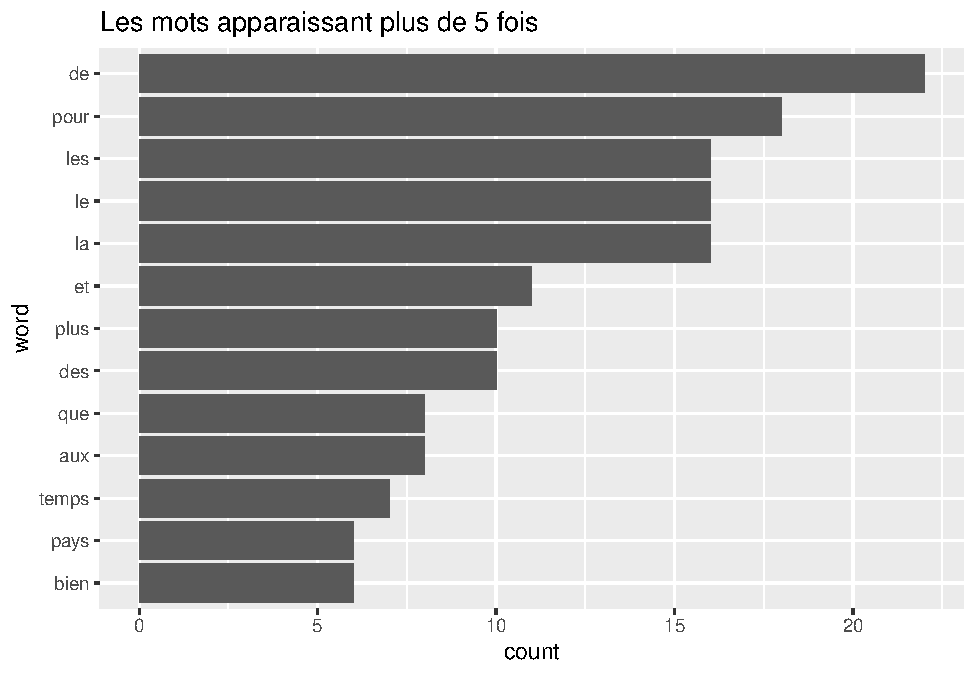
\includegraphics{Texte_mining_files/figure-latex/unnamed-chunk-6-1.pdf}

\begin{Shaded}
\begin{Highlighting}[]
\CommentTok{\# Nombre total de lignes après tokenisation}
\FunctionTok{nrow}\NormalTok{(tokenized\_textes)}
\end{Highlighting}
\end{Shaded}

\begin{verbatim}
## [1] 511
\end{verbatim}

Comme nous pouvons le voir sur le graphique ci-dessus, de nombreux mots
présents n'apportent aucune réelle valeur à notre analyse. Des mots
comme \textbf{de}, \textbf{pour}, \textbf{les}, \textbf{le}, \textbf{la}
sont ce qu'on appelle des mots vides (stop words).

Nous allons supprimer ces mots en utilisant la commande
\emph{anti\_join(stop\_words)}.

\subsubsection{Charger les stop words en
français}\label{charger-les-stop-words-en-franuxe7ais}

\begin{Shaded}
\begin{Highlighting}[]
\NormalTok{stop\_words\_fr }\OtherTok{\textless{}{-}} \FunctionTok{tibble}\NormalTok{(}\AttributeTok{word =} \FunctionTok{stopwords}\NormalTok{(}\StringTok{"fr"}\NormalTok{)) }
\FunctionTok{head}\NormalTok{(stop\_words\_fr)}
\end{Highlighting}
\end{Shaded}

\begin{verbatim}
## # A tibble: 6 x 1
##   word 
##   <chr>
## 1 au   
## 2 aux  
## 3 avec 
## 4 ce   
## 5 ces  
## 6 dans
\end{verbatim}

\begin{Shaded}
\begin{Highlighting}[]
\NormalTok{Stop\_texte }\OtherTok{\textless{}{-}}\NormalTok{ tokenized\_textes }\SpecialCharTok{\%\textgreater{}\%} 
  \FunctionTok{anti\_join}\NormalTok{(stop\_words\_fr, }\AttributeTok{by =} \StringTok{"word"}\NormalTok{)}

\FunctionTok{nrow}\NormalTok{(Stop\_texte)}
\end{Highlighting}
\end{Shaded}

\begin{verbatim}
## [1] 317
\end{verbatim}

On voit bien que le nombre de mots diminue suite à la supression des
stop word

Comme nous pouvons le voir sur le graphique ci-dessous, il reste moins
de mots, mais ils sont beaucoup plus pertinents pour l'analyse.

\begin{Shaded}
\begin{Highlighting}[]
\NormalTok{Stop\_texte }\SpecialCharTok{\%\textgreater{}\%}
  \FunctionTok{anti\_join}\NormalTok{(stop\_words\_fr) }\SpecialCharTok{\%\textgreater{}\%} \CommentTok{\# trouve là où les textes rencontrent des stop words, et les supprime}
  \FunctionTok{count}\NormalTok{(word, }\AttributeTok{sort =} \ConstantTok{TRUE}\NormalTok{) }\SpecialCharTok{\%\textgreater{}\%}
  \FunctionTok{rename}\NormalTok{(}\AttributeTok{count =}\NormalTok{ n) }\SpecialCharTok{\%\textgreater{}\%}
  \FunctionTok{filter}\NormalTok{(count }\SpecialCharTok{\textgreater{}} \DecValTok{5}\NormalTok{) }\SpecialCharTok{\%\textgreater{}\%}
  \FunctionTok{mutate}\NormalTok{(}\AttributeTok{word =} \FunctionTok{reorder}\NormalTok{(word, count)) }\SpecialCharTok{\%\textgreater{}\%}
  \FunctionTok{ggplot}\NormalTok{(}\FunctionTok{aes}\NormalTok{(}\AttributeTok{x =}\NormalTok{ count, }\AttributeTok{y =}\NormalTok{ word)) }\SpecialCharTok{+} 
  \FunctionTok{geom\_col}\NormalTok{() }\SpecialCharTok{+} 
  \FunctionTok{labs}\NormalTok{(}\AttributeTok{title =} \StringTok{"Les mots apparaissant plus de 5 fois"}\NormalTok{) }\SpecialCharTok{+} 
  \FunctionTok{scale\_x\_continuous}\NormalTok{(}\AttributeTok{breaks =} \FunctionTok{seq}\NormalTok{(}\DecValTok{0}\NormalTok{, }\DecValTok{50}\NormalTok{, }\DecValTok{5}\NormalTok{))}
\end{Highlighting}
\end{Shaded}

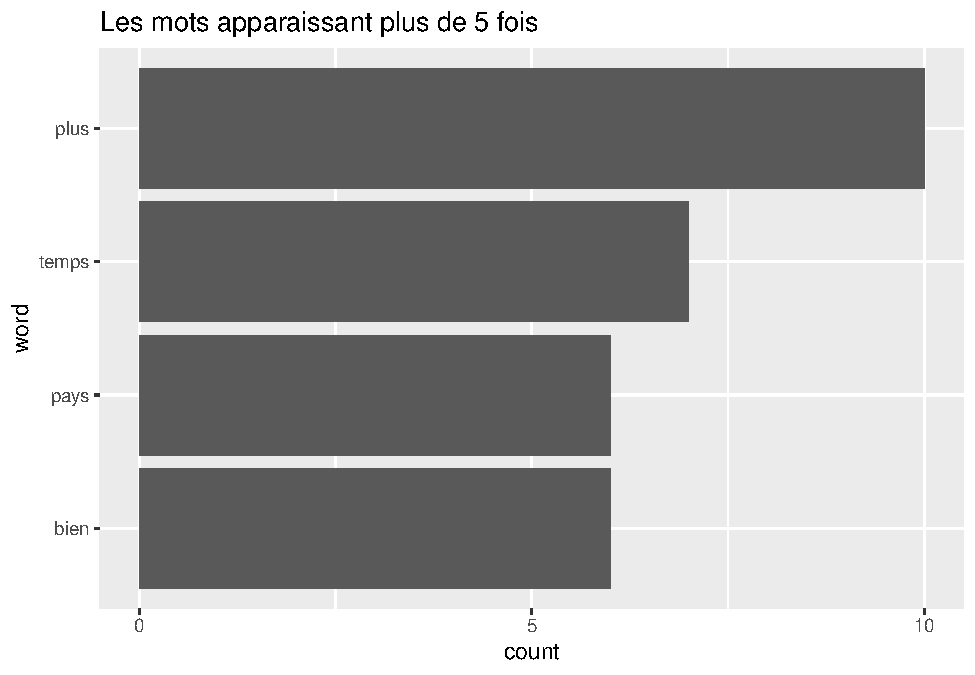
\includegraphics{Texte_mining_files/figure-latex/unnamed-chunk-9-1.pdf}

\begin{Shaded}
\begin{Highlighting}[]
\FunctionTok{library}\NormalTok{(ggwordcloud) }\CommentTok{\# Une autre manière de visualiser}

\NormalTok{Stop\_texte }\SpecialCharTok{\%\textgreater{}\%}
  \FunctionTok{anti\_join}\NormalTok{(stop\_words\_fr) }\SpecialCharTok{\%\textgreater{}\%}
  \FunctionTok{count}\NormalTok{(word, }\AttributeTok{sort =} \ConstantTok{TRUE}\NormalTok{) }\SpecialCharTok{\%\textgreater{}\%}
  \FunctionTok{filter}\NormalTok{(n }\SpecialCharTok{\textgreater{}} \DecValTok{4}\NormalTok{) }\SpecialCharTok{\%\textgreater{}\%}
  \FunctionTok{ggplot}\NormalTok{(}\FunctionTok{aes}\NormalTok{(}\AttributeTok{label =}\NormalTok{ word, }\AttributeTok{size =}\NormalTok{ n, }\AttributeTok{color =}\NormalTok{ n)) }\SpecialCharTok{+} 
  \FunctionTok{geom\_text\_wordcloud}\NormalTok{() }\SpecialCharTok{+} 
  \FunctionTok{scale\_size\_area}\NormalTok{(}\AttributeTok{max\_size =} \DecValTok{15}\NormalTok{) }
\end{Highlighting}
\end{Shaded}

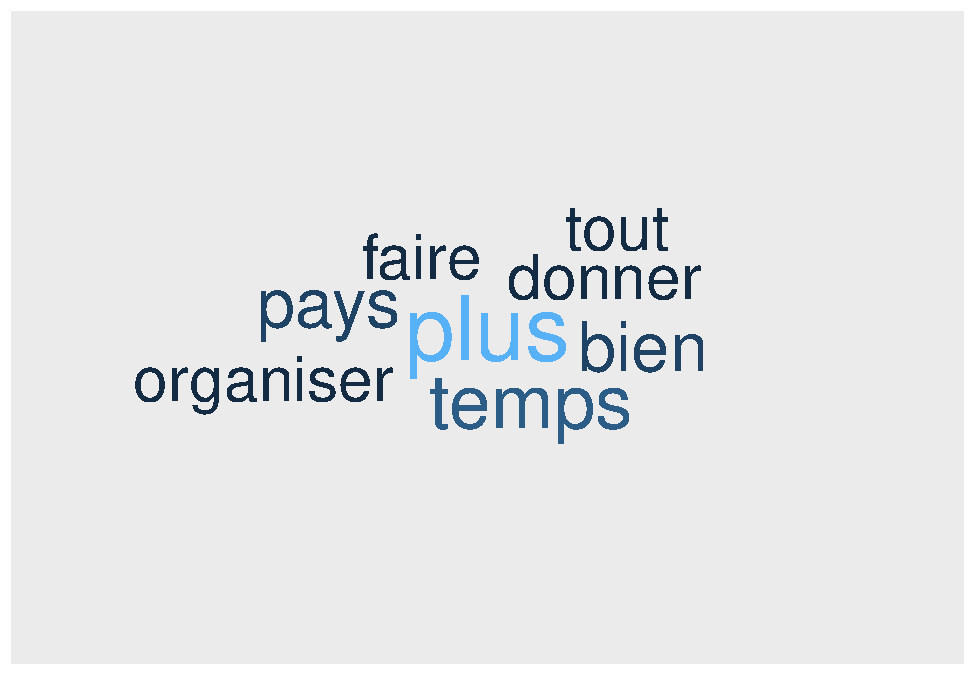
\includegraphics{Texte_mining_files/figure-latex/unnamed-chunk-10-1.pdf}

On peut également voir ci-dessous, la fréquence standard des termes (TF)
pour tous les mots

\begin{Shaded}
\begin{Highlighting}[]
\NormalTok{Stop\_texte }\SpecialCharTok{\%\textgreater{}\%}
  \FunctionTok{count}\NormalTok{(word, }\AttributeTok{sort =} \ConstantTok{TRUE}\NormalTok{) }\SpecialCharTok{\%\textgreater{}\%}
  \FunctionTok{rename}\NormalTok{(}\AttributeTok{count =}\NormalTok{ n) }\SpecialCharTok{\%\textgreater{}\%}
  \FunctionTok{mutate}\NormalTok{(}\AttributeTok{total=}\FunctionTok{sum}\NormalTok{(count))}\SpecialCharTok{\%\textgreater{}\%}
  \FunctionTok{mutate}\NormalTok{(}\AttributeTok{tf=}\NormalTok{count}\SpecialCharTok{/}\NormalTok{total) }\SpecialCharTok{\%\textgreater{}\%}
  \FunctionTok{head}\NormalTok{()}
\end{Highlighting}
\end{Shaded}

\begin{verbatim}
## # A tibble: 6 x 4
##   word   count total     tf
##   <chr>  <int> <int>  <dbl>
## 1 plus      10   317 0.0315
## 2 temps      7   317 0.0221
## 3 bien       6   317 0.0189
## 4 pays       6   317 0.0189
## 5 donner     5   317 0.0158
## 6 faire      5   317 0.0158
\end{verbatim}

L'application des stop word diminue le nombre de mots. Ceci le montre

\begin{Shaded}
\begin{Highlighting}[]
\NormalTok{Stop\_texte }\SpecialCharTok{\%\textgreater{}\%}
  \FunctionTok{count}\NormalTok{(word, }\AttributeTok{sort =} \ConstantTok{TRUE}\NormalTok{)}\SpecialCharTok{\%\textgreater{}\%}
  \FunctionTok{nrow}\NormalTok{()}
\end{Highlighting}
\end{Shaded}

\begin{verbatim}
## [1] 215
\end{verbatim}

\subsubsection{Racinisation}\label{racinisation}

En racinisant, les mots \emph{cultures} et \emph{culture} par exemple se
réduisent en \emph{culture}. Voilà pourquoi le nombre total de mots
diminue comme le résultat de cette commande l'illustre :

\begin{Shaded}
\begin{Highlighting}[]
\CommentTok{\# stemming}
\NormalTok{Stop\_texte }\OtherTok{=}\NormalTok{ Stop\_texte }\SpecialCharTok{\%\textgreater{}\%}
  \FunctionTok{mutate}\NormalTok{(}\AttributeTok{stem =} \FunctionTok{wordStem}\NormalTok{(word))}

\CommentTok{\# unique count of words after stemming}
\NormalTok{Stop\_texte }\SpecialCharTok{\%\textgreater{}\%}
  \FunctionTok{count}\NormalTok{(stem, }\AttributeTok{sort =} \ConstantTok{TRUE}\NormalTok{) }\SpecialCharTok{\%\textgreater{}\%}
  \FunctionTok{nrow}\NormalTok{()}
\end{Highlighting}
\end{Shaded}

\begin{verbatim}
## [1] 201
\end{verbatim}

Fréquence des mots avant le stemming

\begin{Shaded}
\begin{Highlighting}[]
\CommentTok{\# Fréquence des mots avant le stemming}
\NormalTok{Stop\_texte }\SpecialCharTok{\%\textgreater{}\%}
  \FunctionTok{count}\NormalTok{(word) }\SpecialCharTok{\%\textgreater{}\%}
  \FunctionTok{arrange}\NormalTok{(}\FunctionTok{desc}\NormalTok{(n)) }\SpecialCharTok{\%\textgreater{}\%}
  \FunctionTok{head}\NormalTok{(}\DecValTok{10}\NormalTok{)}
\end{Highlighting}
\end{Shaded}

\begin{verbatim}
## # A tibble: 10 x 2
##    word          n
##    <chr>     <int>
##  1 plus         10
##  2 temps         7
##  3 bien          6
##  4 pays          6
##  5 donner        5
##  6 faire         5
##  7 organiser     5
##  8 tout          5
##  9 chaque        4
## 10 culture       4
\end{verbatim}

Fréquence des mots après le stmming

\begin{Shaded}
\begin{Highlighting}[]
\CommentTok{\# Fréquence des mots après le stemming}
\NormalTok{Stop\_texte }\SpecialCharTok{\%\textgreater{}\%}
  \FunctionTok{count}\NormalTok{(stem) }\SpecialCharTok{\%\textgreater{}\%}
  \FunctionTok{arrange}\NormalTok{(}\FunctionTok{desc}\NormalTok{(n)) }\SpecialCharTok{\%\textgreater{}\%}
  \FunctionTok{head}\NormalTok{(}\DecValTok{10}\NormalTok{)}
\end{Highlighting}
\end{Shaded}

\begin{verbatim}
## # A tibble: 10 x 2
##    stem         n
##    <chr>    <int>
##  1 plu         10
##  2 cultur       8
##  3 temp         7
##  4 bien         6
##  5 organis      6
##  6 pai          6
##  7 culturel     5
##  8 donner       5
##  9 fair         5
## 10 journé       5
\end{verbatim}

On remarque que le stemming ne semble pas respecter la logique pour
certains mots. En effet, la racinisation supprime les lettres \emph{s} à
la fin des mots comme \emph{plus} et \emph{temps}. Egalement le mot
\emph{paix} est réduit à \emph{pai}. Cela constitut une limite majeure
quant à la racinisation en langue française. C'est pourquoi dans ce qui
suit, nous ferons fi de cette étape du prétraitement en utilisanat
désormais seulement mes textes issus de l'application des stop word.

\subsubsection{les analyse TF-IDF}\label{les-analyse-tf-idf}

Ci-dessous, nous voyons l'intégralité du tableau TF-IDF. Ce qui nous
intéresse le plus, c'est la colonne tf\_idf, car elle nous donne le
classement pondéré ou l'importance des mots dans notre texte.

\begin{Shaded}
\begin{Highlighting}[]
\NormalTok{texte\_tf\_idf }\OtherTok{\textless{}{-}}\NormalTok{ Stop\_texte }\SpecialCharTok{\%\textgreater{}\%}
  \FunctionTok{count}\NormalTok{(word, id, }\AttributeTok{sort =} \ConstantTok{TRUE}\NormalTok{) }\SpecialCharTok{\%\textgreater{}\%}
  \FunctionTok{rename}\NormalTok{(}\AttributeTok{count =}\NormalTok{ n) }\SpecialCharTok{\%\textgreater{}\%}
  \FunctionTok{bind\_tf\_idf}\NormalTok{(word, id, count)}
\FunctionTok{head}\NormalTok{(texte\_tf\_idf)}
\end{Highlighting}
\end{Shaded}

\begin{verbatim}
## # A tibble: 6 x 6
##   word         id count    tf   idf tf_idf
##   <chr>     <dbl> <int> <dbl> <dbl>  <dbl>
## 1 bien         65     2 0.25   2.20  0.549
## 2 cultures    117     2 0.105  2.71  0.285
## 3 dominante   102     2 0.25   3.81  0.952
## 4 pays         75     2 0.143  2.20  0.314
## 5 tout         32     2 0.222  2.42  0.538
## 6 a            39     1 0.2    3.81  0.761
\end{verbatim}

Les simples décomptes de fréquences de mots peuvent être trompeurs et
peu utiles pour bien comprendre nos données. Il est en fait intéressant
de voir les mots les plus fréquents dans chaque texte.

\begin{Shaded}
\begin{Highlighting}[]
\NormalTok{texte\_tf\_idf }\SpecialCharTok{\%\textgreater{}\%}
  \FunctionTok{select}\NormalTok{(word, id, tf\_idf, count) }\SpecialCharTok{\%\textgreater{}\%}
  \FunctionTok{group\_by}\NormalTok{(id) }\SpecialCharTok{\%\textgreater{}\%}
  \FunctionTok{slice\_max}\NormalTok{(}\AttributeTok{order\_by =}\NormalTok{ count, }\AttributeTok{n =} \DecValTok{6}\NormalTok{, }\AttributeTok{with\_ties=}\ConstantTok{FALSE}\NormalTok{) }\SpecialCharTok{\%\textgreater{}\%} \CommentTok{\#takes top 5 words from each text}
  \FunctionTok{filter}\NormalTok{(id }\SpecialCharTok{\textless{}} \DecValTok{6}\NormalTok{) }\SpecialCharTok{\%\textgreater{}\%} \CommentTok{\#just look at 5 textes}
  \FunctionTok{ggplot}\NormalTok{(}\FunctionTok{aes}\NormalTok{(}\AttributeTok{label =}\NormalTok{ word)) }\SpecialCharTok{+} 
  \FunctionTok{geom\_text\_wordcloud}\NormalTok{() }\SpecialCharTok{+} 
  \FunctionTok{facet\_grid}\NormalTok{(}\AttributeTok{rows =} \FunctionTok{vars}\NormalTok{(id))}
\end{Highlighting}
\end{Shaded}

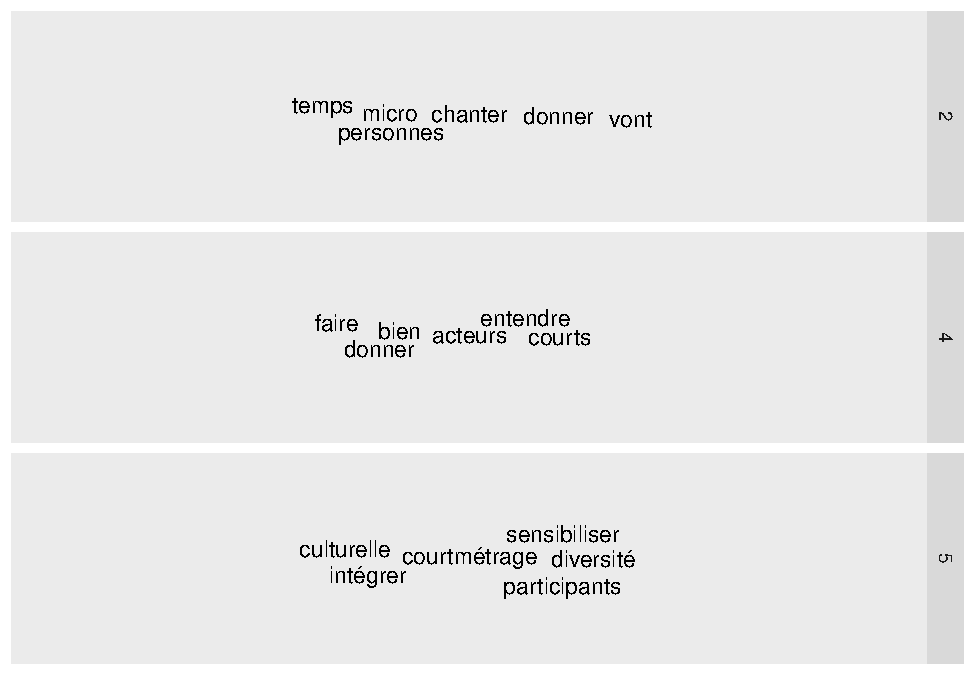
\includegraphics{Texte_mining_files/figure-latex/unnamed-chunk-17-1.pdf}

On s'est limité au cinq premiers textes. Mais les textes correspondant
aux identifiants 1 et 3 sont des NA et donc ont été isolés.

Par ailleurs le résultat qui suit montre aussi qu'il ne faut pas se
limiter à un simple dénombrement des textes mais à leur fréquence.

\begin{Shaded}
\begin{Highlighting}[]
\NormalTok{texte\_tf\_idf }\SpecialCharTok{\%\textgreater{}\%}
  \FunctionTok{select}\NormalTok{(word, id, tf\_idf) }\SpecialCharTok{\%\textgreater{}\%}
  \FunctionTok{group\_by}\NormalTok{(id) }\SpecialCharTok{\%\textgreater{}\%}
  \FunctionTok{slice\_max}\NormalTok{(}\AttributeTok{order\_by =}\NormalTok{ tf\_idf,}\AttributeTok{n =} \DecValTok{6}\NormalTok{, }\AttributeTok{with\_ties=}\ConstantTok{FALSE}\NormalTok{) }\SpecialCharTok{\%\textgreater{}\%} \CommentTok{\#takes top 5 words from each text}
  \FunctionTok{filter}\NormalTok{(id }\SpecialCharTok{\textless{}} \DecValTok{6}\NormalTok{) }\SpecialCharTok{\%\textgreater{}\%} \CommentTok{\#just look at 5 texts}
  \FunctionTok{ggplot}\NormalTok{(}\FunctionTok{aes}\NormalTok{(}\AttributeTok{label =}\NormalTok{ word)) }\SpecialCharTok{+} 
  \FunctionTok{geom\_text\_wordcloud}\NormalTok{() }\SpecialCharTok{+} 
  \FunctionTok{facet\_grid}\NormalTok{(}\AttributeTok{rows =} \FunctionTok{vars}\NormalTok{(id))}
\end{Highlighting}
\end{Shaded}

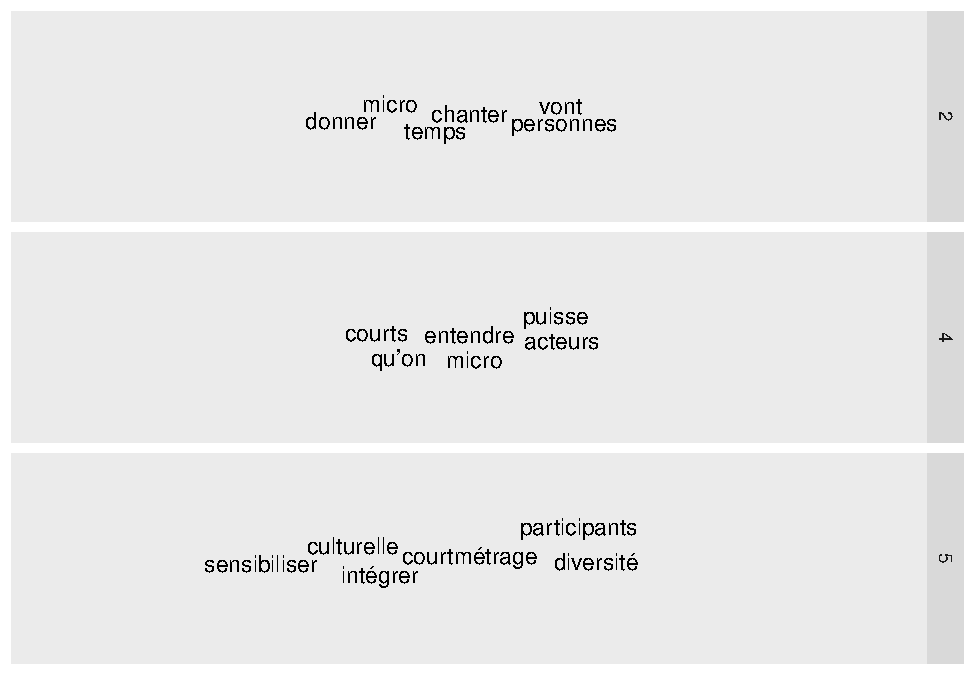
\includegraphics{Texte_mining_files/figure-latex/unnamed-chunk-18-1.pdf}

\subsubsection{Relations entre les mots}\label{relations-entre-les-mots}

Jusqu'à présent, nous avons seulement examiné les mots individuellement.
Mais que faire si nous voulons connaître les relations entre les mots
dans un texte ? Cela peut être accompli grâce aux n-grammes, où n est un
nombre. Auparavant, nous avions effectué une tokenisation mot par mot,
mais nous pouvons aussi tokeniser par groupes de n mots. Créons
maintenant des bigrams (groupes de deux mots) à partir de tous les
textes, puis comptons-les et trions-les.

\begin{Shaded}
\begin{Highlighting}[]
\NormalTok{textes\_bigram }\OtherTok{\textless{}{-}}\NormalTok{ data }\SpecialCharTok{\%\textgreater{}\%}
  \FunctionTok{select}\NormalTok{(id, Texte\_corrige) }\SpecialCharTok{\%\textgreater{}\%}
  \FunctionTok{unnest\_tokens}\NormalTok{(bigram, Texte\_corrige, }\AttributeTok{token =} \StringTok{\textquotesingle{}ngrams\textquotesingle{}}\NormalTok{, }\AttributeTok{n =} \DecValTok{2}\NormalTok{) }
\FunctionTok{head}\NormalTok{(textes\_bigram)}
\end{Highlighting}
\end{Shaded}

\begin{verbatim}
## # A tibble: 6 x 2
##      id bigram       
##   <dbl> <chr>        
## 1     2 donner à     
## 2     2 à temps      
## 3     2 temps le     
## 4     2 le micro     
## 5     2 micro aux    
## 6     2 aux personnes
\end{verbatim}

Comme vous pouvez le voir dans le dataframe ci-dessus, certains
bigrammes contiennent des mots vides (stop words) qui n'apportent pas
beaucoup de valeur. Supprimons ces mots vides. Pour cela, nous allons
d'abord séparer la colonne des bigrammes en deux colonnes distinctes
nommées `word1' et `word2'. Ensuite, nous utiliserons deux fonctions de
filtre pour supprimer les mots vides.

\begin{Shaded}
\begin{Highlighting}[]
\NormalTok{textes\_bigram }\OtherTok{\textless{}{-}}\NormalTok{ textes\_bigram }\SpecialCharTok{\%\textgreater{}\%}
  \FunctionTok{separate}\NormalTok{(bigram, }\FunctionTok{c}\NormalTok{(}\StringTok{"word1"}\NormalTok{, }\StringTok{"word2"}\NormalTok{), }\AttributeTok{sep =} \StringTok{" "}\NormalTok{) }\SpecialCharTok{\%\textgreater{}\%}\CommentTok{\#separates on whitespace}
  \FunctionTok{filter}\NormalTok{(}\SpecialCharTok{!}\NormalTok{word1 }\SpecialCharTok{\%in\%}\NormalTok{ stop\_words\_fr}\SpecialCharTok{$}\NormalTok{word) }\SpecialCharTok{\%\textgreater{}\%}
  \FunctionTok{filter}\NormalTok{(}\SpecialCharTok{!}\NormalTok{word2 }\SpecialCharTok{\%in\%}\NormalTok{ stop\_words\_fr}\SpecialCharTok{$}\NormalTok{word)}

\FunctionTok{head}\NormalTok{(textes\_bigram)}
\end{Highlighting}
\end{Shaded}

\begin{verbatim}
## # A tibble: 6 x 3
##      id word1     word2     
##   <dbl> <chr>     <chr>     
## 1     2 vont      chanter   
## 2     4 sketchs   courts    
## 3     4 bien      donner    
## 4     4 acteurs   qu’on     
## 5     4 qu’on     puisse    
## 6     5 diversité culturelle
\end{verbatim}

On peut maintenant compter les bigram et voir le résultat

\begin{Shaded}
\begin{Highlighting}[]
\NormalTok{bigram\_counts }\OtherTok{\textless{}{-}}\NormalTok{ textes\_bigram }\SpecialCharTok{\%\textgreater{}\%}
  \FunctionTok{count}\NormalTok{(word1, word2, }\AttributeTok{sort =} \ConstantTok{TRUE}\NormalTok{)}
\FunctionTok{head}\NormalTok{(bigram\_counts)}
\end{Highlighting}
\end{Shaded}

\begin{verbatim}
## # A tibble: 6 x 3
##   word1       word2        n
##   <chr>       <chr>    <int>
## 1 chaque      pays         3
## 2 différentes cultures     2
## 3 donner      plus         2
## 4 faut        réduire      2
## 5 plus        grande       2
## 6 soirée      dansante     2
\end{verbatim}

Comme précédemment, on peut aussi créer une mesure TF-IDF avec des
n-grammes. Faisons-le maintenant.

\begin{Shaded}
\begin{Highlighting}[]
\NormalTok{data }\SpecialCharTok{\%\textgreater{}\%}
  \FunctionTok{select}\NormalTok{(id, Texte\_corrige) }\SpecialCharTok{\%\textgreater{}\%}
  \FunctionTok{unnest\_tokens}\NormalTok{(bigram, Texte\_corrige, }\AttributeTok{token =} \StringTok{\textquotesingle{}ngrams\textquotesingle{}}\NormalTok{, }\AttributeTok{n =} \DecValTok{2}\NormalTok{) }\SpecialCharTok{\%\textgreater{}\%}
  \FunctionTok{count}\NormalTok{(id, bigram) }\SpecialCharTok{\%\textgreater{}\%}
  \FunctionTok{bind\_tf\_idf}\NormalTok{(bigram, id, n) }\SpecialCharTok{\%\textgreater{}\%}
  \FunctionTok{group\_by}\NormalTok{(id) }\SpecialCharTok{\%\textgreater{}\%}
  \FunctionTok{arrange}\NormalTok{(id, }\FunctionTok{desc}\NormalTok{(tf\_idf)) }\SpecialCharTok{\%\textgreater{}\%}
  \FunctionTok{head}\NormalTok{()}
\end{Highlighting}
\end{Shaded}

\begin{verbatim}
## # A tibble: 6 x 6
## # Groups:   id [1]
##      id bigram            n    tf   idf tf_idf
##   <dbl> <chr>         <int> <dbl> <dbl>  <dbl>
## 1     2 aux personnes     1 0.111  3.81  0.423
## 2     2 donner à          1 0.111  3.81  0.423
## 3     2 temps le          1 0.111  3.81  0.423
## 4     2 vont chanter      1 0.111  3.81  0.423
## 5     2 à temps           1 0.111  3.81  0.423
## 6     2 personnes qui     1 0.111  3.11  0.346
\end{verbatim}

Comme on peut le voir ci-dessus, beaucoup de valeurs TF-IDF sont
identiques. Cela est en partie dû à la petite taille des textes. Jetons
maintenant un coup d'œil aux relations entre les mots dans tous les
textes, en utilisant un graphe en réseau.

\begin{Shaded}
\begin{Highlighting}[]
\FunctionTok{library}\NormalTok{(}\StringTok{\textquotesingle{}igraph\textquotesingle{}}\NormalTok{)}
\FunctionTok{library}\NormalTok{(}\StringTok{\textquotesingle{}ggraph\textquotesingle{}}\NormalTok{)}
\NormalTok{bi\_graph }\OtherTok{\textless{}{-}}\NormalTok{ bigram\_counts }\SpecialCharTok{\%\textgreater{}\%}
  \FunctionTok{filter}\NormalTok{(n }\SpecialCharTok{\textgreater{}} \DecValTok{1}\NormalTok{) }\SpecialCharTok{\%\textgreater{}\%} 
  \FunctionTok{graph\_from\_data\_frame}\NormalTok{()}

\FunctionTok{ggraph}\NormalTok{(bi\_graph, }\AttributeTok{layout =} \StringTok{"fr"}\NormalTok{) }\SpecialCharTok{+}
  \FunctionTok{geom\_edge\_link}\NormalTok{() }\SpecialCharTok{+}
  \FunctionTok{geom\_node\_point}\NormalTok{() }\SpecialCharTok{+}
  \FunctionTok{geom\_node\_text}\NormalTok{(}\FunctionTok{aes}\NormalTok{(}\AttributeTok{label =}\NormalTok{ name), }\AttributeTok{vjust =} \DecValTok{1}\NormalTok{, }\AttributeTok{hjust =} \DecValTok{1}\NormalTok{)}
\end{Highlighting}
\end{Shaded}

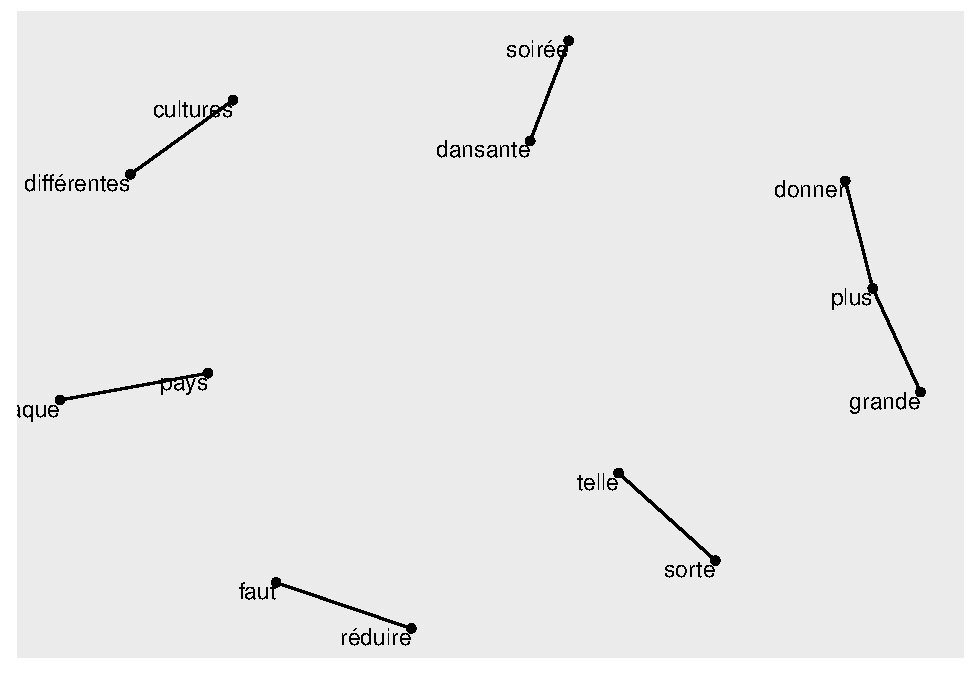
\includegraphics{Texte_mining_files/figure-latex/unnamed-chunk-23-1.pdf}

Comme on peut le voir ci-dessus, de nombreux noms et d'autres
informations ont été extraits des données.

\begin{Shaded}
\begin{Highlighting}[]
\NormalTok{texte\_trigram }\OtherTok{\textless{}{-}}\NormalTok{ data }\SpecialCharTok{\%\textgreater{}\%}
  \FunctionTok{select}\NormalTok{(id, Texte\_corrige) }\SpecialCharTok{\%\textgreater{}\%}
  \FunctionTok{unnest\_tokens}\NormalTok{(trigram, Texte\_corrige, }\AttributeTok{token =} \StringTok{\textquotesingle{}ngrams\textquotesingle{}}\NormalTok{, }\AttributeTok{n =} \DecValTok{3}\NormalTok{) }\SpecialCharTok{\%\textgreater{}\%}
  \FunctionTok{separate}\NormalTok{(trigram, }\FunctionTok{c}\NormalTok{(}\StringTok{"word1"}\NormalTok{, }\StringTok{"word2"}\NormalTok{, }\StringTok{"word3"}\NormalTok{), }\AttributeTok{sep =} \StringTok{" "}\NormalTok{) }\SpecialCharTok{\%\textgreater{}\%} \CommentTok{\#separates on whitespace}
  \FunctionTok{filter}\NormalTok{(}\SpecialCharTok{!}\NormalTok{word1 }\SpecialCharTok{\%in\%}\NormalTok{ stop\_words\_fr}\SpecialCharTok{$}\NormalTok{word) }\SpecialCharTok{\%\textgreater{}\%}
  \FunctionTok{filter}\NormalTok{(}\SpecialCharTok{!}\NormalTok{word2 }\SpecialCharTok{\%in\%}\NormalTok{ stop\_words\_fr}\SpecialCharTok{$}\NormalTok{word) }\SpecialCharTok{\%\textgreater{}\%}
  \FunctionTok{filter}\NormalTok{(}\SpecialCharTok{!}\NormalTok{word3 }\SpecialCharTok{\%in\%}\NormalTok{ stop\_words\_fr}\SpecialCharTok{$}\NormalTok{word)}

\FunctionTok{head}\NormalTok{(texte\_trigram)}
\end{Highlighting}
\end{Shaded}

\begin{verbatim}
## # A tibble: 6 x 4
##      id word1        word2          word3          
##   <dbl> <chr>        <chr>          <chr>          
## 1     4 acteurs      qu’on          puisse         
## 2     7 scène        car            habituellement 
## 3    11 meilleure    sonorisation   côté           
## 4    11 sonorisation côté           technique      
## 5    14 dautres      journées       continuellement
## 6    14 favoriser    lapprentissage culturel
\end{verbatim}

On peut aussi compter les trigram et voir le résultat

\begin{Shaded}
\begin{Highlighting}[]
\NormalTok{trigram\_counts }\OtherTok{\textless{}{-}}\NormalTok{ texte\_trigram }\SpecialCharTok{\%\textgreater{}\%}
  \FunctionTok{count}\NormalTok{(word1, word2, word3, }\AttributeTok{sort =} \ConstantTok{TRUE}\NormalTok{)}
\FunctionTok{head}\NormalTok{(trigram\_counts)}
\end{Highlighting}
\end{Shaded}

\begin{verbatim}
## # A tibble: 6 x 4
##   word1    word2     word3            n
##   <chr>    <chr>     <chr>        <int>
## 1 acteurs  qu’on     puisse           1
## 2 ajouter  plus      d’activités      1
## 3 aménager plus      despace          1
## 4 bien     organiser l’événement      1
## 5 car      c’est     souvent          1
## 6 certains modules   statistiques     1
\end{verbatim}

Comme précédemment, on peut aussi créer une mesure TF-IDF avec des
trigrammes. Faisons-le maintenant.

\begin{Shaded}
\begin{Highlighting}[]
\NormalTok{data }\SpecialCharTok{\%\textgreater{}\%}
  \FunctionTok{select}\NormalTok{(id, Texte\_corrige) }\SpecialCharTok{\%\textgreater{}\%}
  \FunctionTok{unnest\_tokens}\NormalTok{(trigram, Texte\_corrige, }\AttributeTok{token =} \StringTok{\textquotesingle{}ngrams\textquotesingle{}}\NormalTok{, }\AttributeTok{n =} \DecValTok{3}\NormalTok{) }\SpecialCharTok{\%\textgreater{}\%}
  \FunctionTok{count}\NormalTok{(id, trigram) }\SpecialCharTok{\%\textgreater{}\%}
  \FunctionTok{bind\_tf\_idf}\NormalTok{(trigram, id, n) }\SpecialCharTok{\%\textgreater{}\%}
  \FunctionTok{group\_by}\NormalTok{(id) }\SpecialCharTok{\%\textgreater{}\%}
  \FunctionTok{arrange}\NormalTok{(id, }\FunctionTok{desc}\NormalTok{(tf\_idf)) }\SpecialCharTok{\%\textgreater{}\%}
  \FunctionTok{head}\NormalTok{()}
\end{Highlighting}
\end{Shaded}

\begin{verbatim}
## # A tibble: 6 x 6
## # Groups:   id [1]
##      id trigram                 n    tf   idf tf_idf
##   <dbl> <chr>               <int> <dbl> <dbl>  <dbl>
## 1     2 aux personnes qui       1 0.125  3.81  0.476
## 2     2 donner à temps          1 0.125  3.81  0.476
## 3     2 micro aux personnes     1 0.125  3.81  0.476
## 4     2 personnes qui vont      1 0.125  3.81  0.476
## 5     2 qui vont chanter        1 0.125  3.81  0.476
## 6     2 temps le micro          1 0.125  3.81  0.476
\end{verbatim}

Comme on peut le voir ci-dessus, beaucoup de valeurs TF-IDF sont
identiques. Cela est en partie dû à la petite taille des textes comme
remarqué dans le cas bigram. Jetons maintenant un coup d'œil aux
relations entre les mots dans l'ensemble des textes, en utilisant un
graphe en réseau.

\begin{Shaded}
\begin{Highlighting}[]
\NormalTok{tri\_graph }\OtherTok{\textless{}{-}}\NormalTok{ trigram\_counts }\SpecialCharTok{\%\textgreater{}\%}
  \FunctionTok{filter}\NormalTok{(n }\SpecialCharTok{\textgreater{}} \DecValTok{0}\NormalTok{) }\SpecialCharTok{\%\textgreater{}\%} \CommentTok{\# Ici, on garde TOUS les trigrammes présents au moins une fois}
  \FunctionTok{graph\_from\_data\_frame}\NormalTok{()}

\FunctionTok{ggraph}\NormalTok{(tri\_graph, }\AttributeTok{layout =} \StringTok{"fr"}\NormalTok{) }\SpecialCharTok{+}
  \FunctionTok{geom\_edge\_link}\NormalTok{() }\SpecialCharTok{+}
  \FunctionTok{geom\_node\_point}\NormalTok{() }\SpecialCharTok{+}
  \FunctionTok{geom\_node\_text}\NormalTok{(}\FunctionTok{aes}\NormalTok{(}\AttributeTok{label =}\NormalTok{ name), }\AttributeTok{vjust =} \DecValTok{1}\NormalTok{, }\AttributeTok{hjust =} \DecValTok{1}\NormalTok{)}
\end{Highlighting}
\end{Shaded}

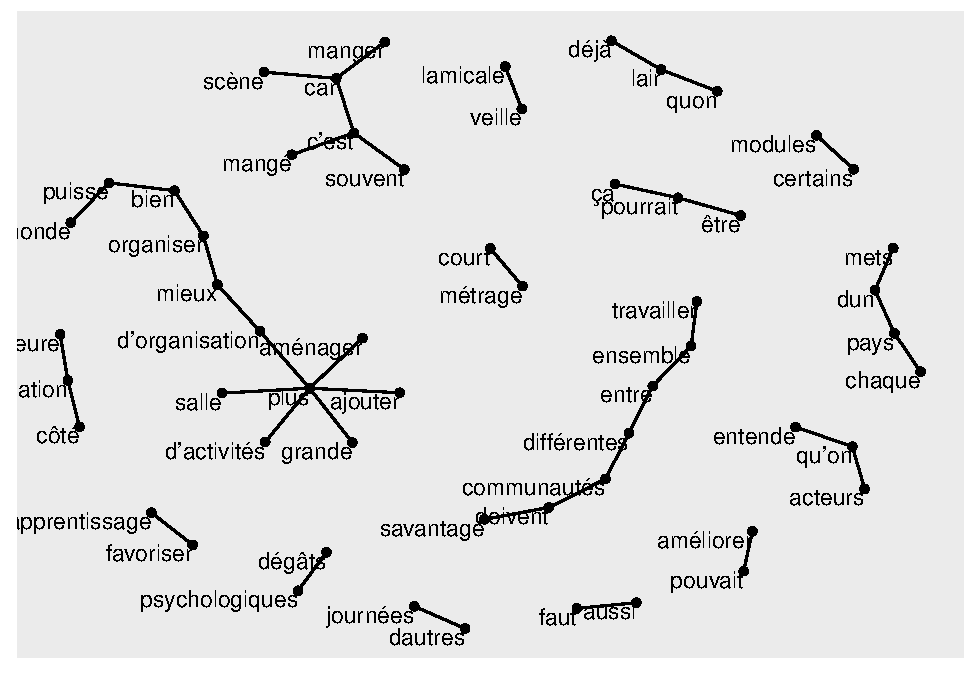
\includegraphics{Texte_mining_files/figure-latex/unnamed-chunk-27-1.pdf}

Normalement, on mettrait n \textgreater{} 1 ou n \textgreater{} 2 pour
filtrer les trigrammes peu fréquents, mais dans notre cas, les textets
sont très courts, donc les trigrammes se répètent très peu.

*Résultat : quasiment aucun trigramme n'apparaît plus d'une fois. Du
coup, si on filtre avec n \textgreater{} 1 ou n \textgreater{} 2 → le
graphe devient vide (aucun trigramme à afficher).

En mettant n \textgreater{} 0, on garde tous les trigrammes possibles,
même ceux présents une seule fois. Cela permet d'obtenir un graphe, même
si les connexions sont faibles (juste 1 apparition).

Dans notre base de données, le champ contenant les suggestions n'est pas
obligatoire, ce qui signifie que plusieurs enregistrements présentent
des valeurs manquantes (NA). Lors de l'application initiale du modèle
LDA sur l'ensemble de la base, nous avons constaté que certains textes
vides étaient malgré tout classés dans une catégorie, simplement parce
qu'ils étaient présents dans les données en entrée. En d'autres termes,
le modèle attribuait un sujet à un champ vide, ce qui n'a pas de sens et
fausse l'interprétation : dans la nouvelle variable contenant les
catégories issues du LDA, on retrouvait ainsi des lignes avec un texte
vide associé à une thématique, comme si le modèle avait `catégorisé du
vide'.

Pour éviter ce biais, nous avons adopté une nouvelle approche plus
rigoureuse. Nous avons d'abord isolé les textes non vides, c'est-à-dire
les enregistrements contenant effectivement une suggestion. Le modèle
LDA a donc été appliqué uniquement sur cette sous-base, ce qui garantit
que chaque catégorisation repose sur un contenu textuel réel.

En parallèle, nous avons soigneusement conservé les identifiants (IDs)
des textes vides, afin de pouvoir les réintégrer dans la base complète
après classification. Cela permet de reconstituer une base cohérente, où
:

\begin{itemize}
\item
  -les textes contenant une suggestion sont associés à une catégorie
  issue du LDA,
\item
  -les textes vides conservent leur place, avec éventuellement une
  étiquette neutre comme `Non renseigné' ou NA dans la variable de
  catégorie.
\end{itemize}

Cette méthode permet ainsi de respecter la structure initiale de la
base, d'éviter des classifications erronées sur des données absentes, et
de garantir une analyse fiable et interprétable.

\begin{Shaded}
\begin{Highlighting}[]
\CommentTok{\# 1. Extraire les ID avant prétraitement (Texte\_JI)}
\NormalTok{Id\_initial\_texte }\OtherTok{\textless{}{-}} \FunctionTok{unique}\NormalTok{(Texte\_JI}\SpecialCharTok{$}\NormalTok{id)}
\FunctionTok{length}\NormalTok{(Id\_initial\_texte)}
\end{Highlighting}
\end{Shaded}

\begin{verbatim}
## [1] 128
\end{verbatim}

\begin{Shaded}
\begin{Highlighting}[]
\CommentTok{\# 2. Extraire les ID après prétraitement (Stop\_texte)}
\NormalTok{Id\_final\_texte }\OtherTok{\textless{}{-}} \FunctionTok{unique}\NormalTok{(Stop\_texte}\SpecialCharTok{$}\NormalTok{id)}
\FunctionTok{length}\NormalTok{(Id\_final\_texte)}
\end{Highlighting}
\end{Shaded}

\begin{verbatim}
## [1] 45
\end{verbatim}

\begin{Shaded}
\begin{Highlighting}[]
\CommentTok{\#. Identifier les tweets manquants (présents avant, absents après)}
\NormalTok{Id\_texte\_NA }\OtherTok{\textless{}{-}} \FunctionTok{setdiff}\NormalTok{(Id\_initial\_texte, Id\_final\_texte)}
\FunctionTok{length}\NormalTok{(Id\_texte\_NA)}
\end{Highlighting}
\end{Shaded}

\begin{verbatim}
## [1] 83
\end{verbatim}

\section{3. Analyse Thématique (LDA)}\label{sec:importation}

Il est courant d'avoir une collection de documents, comme des articles
de presse ou des publications sur les réseaux sociaux, que l'on souhaite
diviser en thèmes. Autrement dit, on veut savoir quel est le sujet
principal dans chaque document. Cela peut se faire grâce à une technique
appelée modélisation thématique (topic modeling). Ici, nous allons
explorer la modélisation thématique à travers la méthode LDA (Latent
Dirichlet Allocation).

LDA repose sur deux grands principes : Chaque document est un mélange de
plusieurs sujets

Chaque sujet est un mélange de mots

Un exemple classique serait de supposer qu'il existe deux grands sujets
dans les actualités : la politique et le divertissement. Le sujet
politique contiendra des mots comme élu, gouvernement,

Tandis que le sujet divertissement contiendra des mots comme film,
acteur. Mais certains mots peuvent apparaître dans les deux, comme prix
ou budget.

LDA va identifier : les mélanges de mots qui composent chaque sujet, et
les mélanges de sujets qui composent chaque document. Voyons cela à
travers un exemple : On commence par créer notre modèle LDA. La fonction
LDA() nécessite en entrée une matrice document-terme
(DocumentTermMatrix), que l'on peut créer à partir de notre base déjà
prétraitée que nous avons généré précédemment.

\subsubsection{Création d'une matrice
document-thème}\label{cruxe9ation-dune-matrice-document-thuxe8me}

\begin{Shaded}
\begin{Highlighting}[]
\CommentTok{\# création d\textquotesingle{}une matrice document{-}thème pour LDA}
\NormalTok{df\_dtm }\OtherTok{\textless{}{-}}\NormalTok{ Stop\_texte }\SpecialCharTok{\%\textgreater{}\%}
  \FunctionTok{count}\NormalTok{(id, word) }\SpecialCharTok{\%\textgreater{}\%}              
  \FunctionTok{cast\_dtm}\NormalTok{(id, word, n)  }
\end{Highlighting}
\end{Shaded}

\subsection{Choix du nombre k de
thèmes}\label{choix-du-nombre-k-de-thuxe8mes}

Dans le cadre de la modélisation thématique avec LDA (Latent Dirichlet
Allocation), un des éléments clés du paramétrage est le choix du nombre
de thèmes (K). Ce paramètre n'est pas déterminé automatiquement par le
modèle ; il doit être choisi par l'utilisateur, en fonction des données
et des objectifs de l'analyse. Or, le nombre de thèmes a un impact
direct sur la qualité et la lisibilité du modèle :

Un K trop petit risque de regrouper des thématiques très différentes
dans un même sujet, rendant le résultat peu précis.

Un K trop grand peut sur-segmenter les données, en produisant des thèmes
trop spécifiques ou redondants, souvent difficiles à interpréter.

C'est pourquoi il est important de trouver un équilibre, c'est-à-dire un
K optimal qui capte suffisamment de variété sans trop complexifier le
modèle.

Afin de déterminer lenombre K optimal de thèmes, on utilisons la
perplexité du modèle pour plusieurs valeurs de K La perplexité est une
mesure standard issue de la modélisation probabiliste, souvent utilisée
pour évaluer les modèles de langage. Dans le contexte de LDA, elle
mesure dans quelle mesure le modèle `explique' les données textuelles

\begin{Shaded}
\begin{Highlighting}[]
\NormalTok{k\_values }\OtherTok{\textless{}{-}} \DecValTok{2}\SpecialCharTok{:}\DecValTok{10}
\NormalTok{perplexities }\OtherTok{\textless{}{-}} \FunctionTok{sapply}\NormalTok{(k\_values, }\ControlFlowTok{function}\NormalTok{(k) \{}
\NormalTok{  lda\_model }\OtherTok{\textless{}{-}} \FunctionTok{LDA}\NormalTok{(df\_dtm, }\AttributeTok{k =}\NormalTok{ k, }\AttributeTok{control =} \FunctionTok{list}\NormalTok{(}\AttributeTok{seed =} \DecValTok{1234}\NormalTok{))}
  \FunctionTok{perplexity}\NormalTok{(lda\_model)}
\NormalTok{\})}

\CommentTok{\# Afficher le graphique}
\FunctionTok{ggplot}\NormalTok{(}\FunctionTok{data.frame}\NormalTok{(}\AttributeTok{K =}\NormalTok{ k\_values, }\AttributeTok{Perplexity =}\NormalTok{ perplexities), }\FunctionTok{aes}\NormalTok{(}\AttributeTok{x =}\NormalTok{ K, }\AttributeTok{y =}\NormalTok{ Perplexity)) }\SpecialCharTok{+}
  \FunctionTok{geom\_point}\NormalTok{() }\SpecialCharTok{+} \FunctionTok{geom\_line}\NormalTok{() }\SpecialCharTok{+}
  \FunctionTok{labs}\NormalTok{(}\AttributeTok{title =} \StringTok{"Choix du K optimal avec la perplexité"}\NormalTok{,}
       \AttributeTok{x =} \StringTok{"Nombre de thèmes (K)"}\NormalTok{, }\AttributeTok{y =} \StringTok{"Perplexité"}\NormalTok{)}
\end{Highlighting}
\end{Shaded}

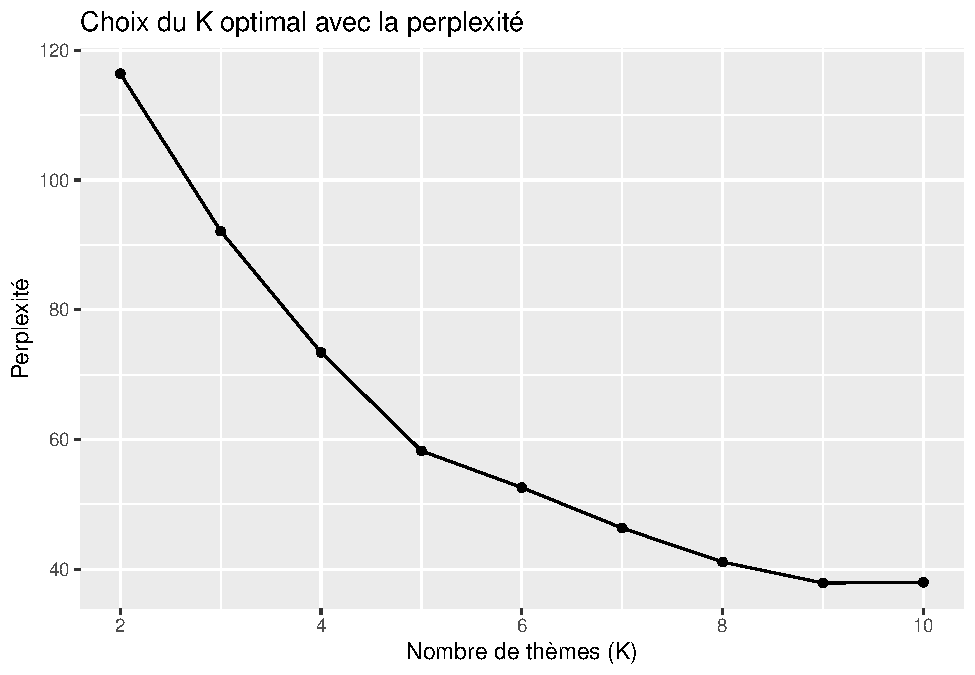
\includegraphics{Texte_mining_files/figure-latex/unnamed-chunk-30-1.pdf}

Le graphique montre une forte diminution de la perplexité entre K = 2 et
K = 7, ce qui indique que chaque thème ajouté dans cette plage apporte
une réelle amélioration du modèle. Ensuite, à partir de K ≈ 8, la courbe
commence à s'aplatir : les gains supplémentaires deviennent de plus en
plus faibles.

Ce comportement suggère qu'à partir de K = 8, ajouter davantage de
thèmes n'améliore plus significativement la qualité du modèle, tout en
augmentant sa complexité. On peut donc considérer K = 8 comme un bon
compromis, car il permet de capter une diversité raisonnable de
thématiques sans trop fragmenter les données.

Cela justifie donc le choix de 8 thèmes comme valeur optimale dans notre
modélisation LDA.

\paragraph{Généralement}\label{guxe9nuxe9ralement}

En théorie, la perplexité est censée diminuer à mesure que le nombre de
thèmes (K) augmente. En effet, un modèle avec plus de thèmes dispose de
plus de `flexibilité' pour représenter les textes de manière fine. Cela
se traduit généralement par une meilleure capacité à prédire les mots
observés dans les documents --- donc une perplexité plus faible.

Cependant, ce comportement n'est pas garanti dans tous les cas. Il peut
arriver que la perplexité stagne voire augmente à partir d'un certain K,
ou ne suive pas une baisse régulière. Ce phénomène peut être lié à
plusieurs facteurs, notamment à la nature des textes analysés.

Un cas courant :

Les mots utilisés dans les documents peuvent être très variés même s'ils
expriment des idées similaires. Par exemple, des mots comme
\textbf{gouvernement}, \textbf{État}, \textbf{autorités},
\textbf{institution} peuvent tous renvoyer à la même notion politique,
mais être traités comme des termes distincts par le modèle. Cela peut
fragmenter artificiellement les thèmes, ou faire croire à une diversité
de contenus plus grande qu'en réalité.

Dans ces situations, la perplexité peut ne plus refléter fidèlement la
\textbf{cohérence sémantique} des thèmes. Elle devient donc une mesure
limitée, surtout si les textes sont courts, informels ou s'ils
contiennent beaucoup de synonymes ou paraphrases.

\subsubsection{Une solution souvent utilisée : Groupage par
thème}\label{une-solution-souvent-utilisuxe9e-groupage-par-thuxe8me}

\begin{Shaded}
\begin{Highlighting}[]
\NormalTok{text\_df2 }\OtherTok{\textless{}{-}}\NormalTok{ Stop\_texte }\SpecialCharTok{\%\textgreater{}\%}
  \FunctionTok{mutate}\NormalTok{(}\AttributeTok{text\_semantic =}\NormalTok{ word) }\SpecialCharTok{\%\textgreater{}\%}  \CommentTok{\# dupliquer la colonne lemmatisée}
  \FunctionTok{mutate}\NormalTok{(}
    \AttributeTok{text\_semantic =} \FunctionTok{str\_replace\_all}\NormalTok{(text\_semantic, }\StringTok{"}\SpecialCharTok{\textbackslash{}\textbackslash{}}\StringTok{b(manger|plat|mets|piment|restaurant)}\SpecialCharTok{\textbackslash{}\textbackslash{}}\StringTok{b"}\NormalTok{, }\StringTok{"alimentation"}\NormalTok{),}
    \AttributeTok{text\_semantic =} \FunctionTok{str\_replace\_all}\NormalTok{(text\_semantic, }\StringTok{"}\SpecialCharTok{\textbackslash{}\textbackslash{}}\StringTok{b(sketch|micro|temps|chanter|court|courtmétrage|sketcheval|scène|culture|culturel|lapprentissage|salle|présentation|apprendre|discours|métrage|fun|espace|prestataire|marrant|comique|communauté|aménager)}\SpecialCharTok{\textbackslash{}\textbackslash{}}\StringTok{b"}\NormalTok{, }\StringTok{"animation"}\NormalTok{),}
    \AttributeTok{text\_semantic =} \FunctionTok{str\_replace\_all}\NormalTok{(text\_semantic, }\StringTok{"}\SpecialCharTok{\textbackslash{}\textbackslash{}}\StringTok{b(audible|sonorisation|technique)}\SpecialCharTok{\textbackslash{}\textbackslash{}}\StringTok{b"}\NormalTok{, }\StringTok{"technique"}\NormalTok{),}
    \AttributeTok{text\_semantic =} \FunctionTok{str\_replace\_all}\NormalTok{(text\_semantic, }\StringTok{"}\SpecialCharTok{\textbackslash{}\textbackslash{}}\StringTok{b(communication|organisation|créativité|organiser)}\SpecialCharTok{\textbackslash{}\textbackslash{}}\StringTok{b"}\NormalTok{, }\StringTok{"Organisation"}\NormalTok{)}
\NormalTok{  )}
\end{Highlighting}
\end{Shaded}

\subsubsection{Limites : pas trop flexible surtout en cas de grands
volumes de
données}\label{limites-pas-trop-flexible-surtout-en-cas-de-grands-volumes-de-donnuxe9es}

Dans ce qui suit, nous continuerons directement avec les données déjà
prétraitées et visualisées sans appliquer un groupage supplémentaire.

\begin{Shaded}
\begin{Highlighting}[]
\NormalTok{lda\_model }\OtherTok{\textless{}{-}} \FunctionTok{LDA}\NormalTok{(df\_dtm, }\AttributeTok{k =} \DecValTok{8}\NormalTok{, }\AttributeTok{control =} \FunctionTok{list}\NormalTok{(}\AttributeTok{seed =} \DecValTok{1234}\NormalTok{))}

\CommentTok{\# Termes par thème}
\NormalTok{terms\_by\_topic }\OtherTok{\textless{}{-}} \FunctionTok{tidy}\NormalTok{(lda\_model, }\AttributeTok{matrix =} \StringTok{"beta"}\NormalTok{)}
\NormalTok{terms\_by\_topic}
\end{Highlighting}
\end{Shaded}

\begin{verbatim}
## # A tibble: 1,720 x 3
##    topic term         beta
##    <int> <chr>       <dbl>
##  1     1 chanter 5.02e-154
##  2     2 chanter 4.94e-324
##  3     3 chanter 5.02e-154
##  4     4 chanter 1.88e-154
##  5     5 chanter 1.81e-  2
##  6     6 chanter 3.48e-154
##  7     7 chanter 2.77e-154
##  8     8 chanter 1.88e-154
##  9     1 donner  1.14e-153
## 10     2 donner  4.88e-  2
## # i 1,710 more rows
\end{verbatim}

La colonne beta représente la probabilité qu'un mot donné appartienne à
un thème particulier. En d'autres termes, plus la valeur de beta est
élevée pour un mot dans un thème, plus ce mot est représentatif de ce
thème

\begin{Shaded}
\begin{Highlighting}[]
\NormalTok{top\_terms }\OtherTok{\textless{}{-}}\NormalTok{ terms\_by\_topic }\SpecialCharTok{\%\textgreater{}\%}
  \FunctionTok{group\_by}\NormalTok{(topic) }\SpecialCharTok{\%\textgreater{}\%}
  \FunctionTok{slice\_max}\NormalTok{(beta, }\AttributeTok{n =} \DecValTok{10}\NormalTok{, }\AttributeTok{with\_ties =} \ConstantTok{FALSE}\NormalTok{) }\SpecialCharTok{\%\textgreater{}\%}  \CommentTok{\# Prend exactement 10 termes par thème}
  \FunctionTok{ungroup}\NormalTok{() }\SpecialCharTok{\%\textgreater{}\%}
  \FunctionTok{arrange}\NormalTok{(topic, }\SpecialCharTok{{-}}\NormalTok{beta)  }\CommentTok{\# Trie par thème et par probabilité décroissante}

\CommentTok{\# Vérification du nombre de termes sélectionnés par thème}
\NormalTok{top\_terms }\SpecialCharTok{\%\textgreater{}\%}
  \FunctionTok{count}\NormalTok{(topic) }
\end{Highlighting}
\end{Shaded}

\begin{verbatim}
## # A tibble: 8 x 2
##   topic     n
##   <int> <int>
## 1     1    10
## 2     2    10
## 3     3    10
## 4     4    10
## 5     5    10
## 6     6    10
## 7     7    10
## 8     8    10
\end{verbatim}

1O termes ont été sélectionnés par thèmes. On peut les visualiser
également

\begin{Shaded}
\begin{Highlighting}[]
\NormalTok{top\_terms }\SpecialCharTok{\%\textgreater{}\%}
  \FunctionTok{mutate}\NormalTok{(}\AttributeTok{term =} \FunctionTok{reorder\_within}\NormalTok{(term, beta, topic)) }\SpecialCharTok{\%\textgreater{}\%}
  \FunctionTok{ggplot}\NormalTok{(}\FunctionTok{aes}\NormalTok{(beta, term, }\AttributeTok{fill =} \FunctionTok{factor}\NormalTok{(topic))) }\SpecialCharTok{+}
  \FunctionTok{geom\_col}\NormalTok{(}\AttributeTok{show.legend =} \ConstantTok{FALSE}\NormalTok{) }\SpecialCharTok{+}
  \FunctionTok{facet\_wrap}\NormalTok{(}\SpecialCharTok{\textasciitilde{}}\NormalTok{ topic, }\AttributeTok{scales =} \StringTok{"free"}\NormalTok{) }\SpecialCharTok{+}
  \FunctionTok{scale\_y\_reordered}\NormalTok{() }\SpecialCharTok{+}
  \FunctionTok{labs}\NormalTok{(}\AttributeTok{title =} \StringTok{"Termes les plus probables par thème"}\NormalTok{,}
       \AttributeTok{x =} \StringTok{"Probabilité (beta)"}\NormalTok{, }\AttributeTok{y =} \StringTok{"Terme"}\NormalTok{)}
\end{Highlighting}
\end{Shaded}

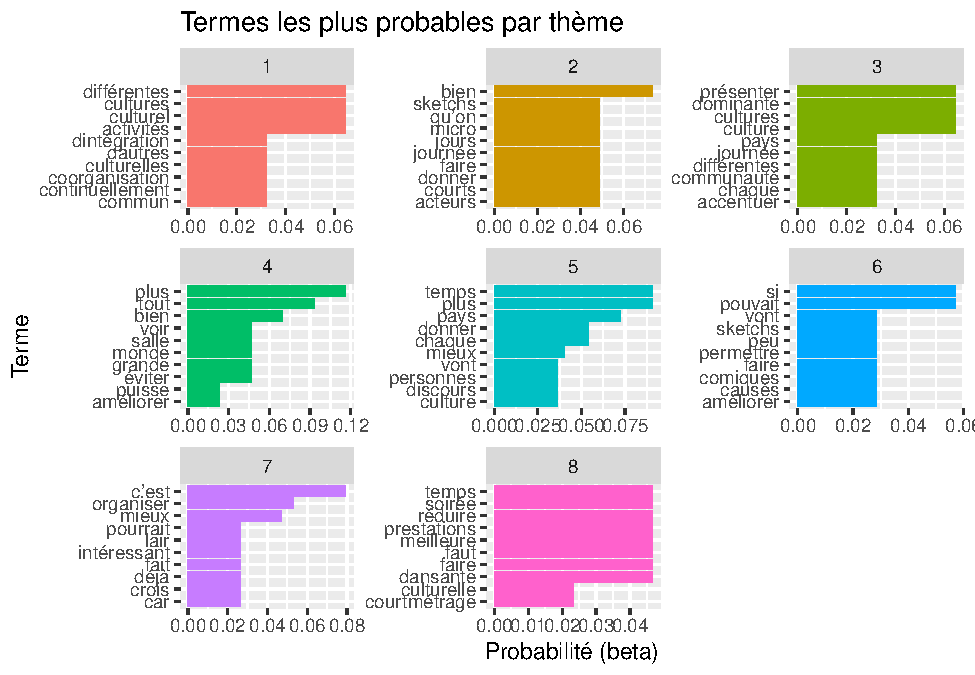
\includegraphics{Texte_mining_files/figure-latex/unnamed-chunk-34-1.pdf}

\begin{Shaded}
\begin{Highlighting}[]
\CommentTok{\# Étape 4 : Classification des textes par thème}
\NormalTok{textes\_gamma }\OtherTok{\textless{}{-}} \FunctionTok{tidy}\NormalTok{(lda\_model, }\AttributeTok{matrix =} \StringTok{"gamma"}\NormalTok{)}
\CommentTok{\# Afficher les textes avec leur thème dominant}
\NormalTok{textes\_classified }\OtherTok{\textless{}{-}}\NormalTok{ textes\_gamma }\SpecialCharTok{\%\textgreater{}\%}
  \FunctionTok{group\_by}\NormalTok{(document) }\SpecialCharTok{\%\textgreater{}\%}
  \FunctionTok{slice\_max}\NormalTok{(gamma) }\SpecialCharTok{\%\textgreater{}\%}
  \FunctionTok{ungroup}\NormalTok{()}
\end{Highlighting}
\end{Shaded}

Ici pour chaque texte, on peut voir la probabilité qu'il a d'appartenir
à chacun des thèmes.

\begin{Shaded}
\begin{Highlighting}[]
\CommentTok{\# Nombre de texte dans chaque thème}
\NormalTok{textes\_classified }\SpecialCharTok{\%\textgreater{}\%}
  \FunctionTok{count}\NormalTok{(topic)}
\end{Highlighting}
\end{Shaded}

\begin{verbatim}
## # A tibble: 8 x 2
##   topic     n
##   <int> <int>
## 1     1     3
## 2     2     6
## 3     3     3
## 4     4     7
## 5     5     8
## 6     6     3
## 7     7     5
## 8     8    10
\end{verbatim}

Pour chaque thème, on voit le nombre de textes

\begin{Shaded}
\begin{Highlighting}[]
\CommentTok{\# Visualisation des nombres de texte dans chaque thème}
\NormalTok{textes\_classified }\SpecialCharTok{\%\textgreater{}\%}
  \FunctionTok{ggplot}\NormalTok{(}\FunctionTok{aes}\NormalTok{(}\FunctionTok{factor}\NormalTok{(topic), }\AttributeTok{fill =} \FunctionTok{factor}\NormalTok{(topic))) }\SpecialCharTok{+}
  \FunctionTok{geom\_bar}\NormalTok{() }\SpecialCharTok{+}
  \FunctionTok{labs}\NormalTok{(}\AttributeTok{title =} \StringTok{"Distribution des thèmes dominants"}\NormalTok{,}
       \AttributeTok{x =} \StringTok{"Thème"}\NormalTok{, }\AttributeTok{y =} \StringTok{"Nombre de textes"}\NormalTok{)}
\end{Highlighting}
\end{Shaded}

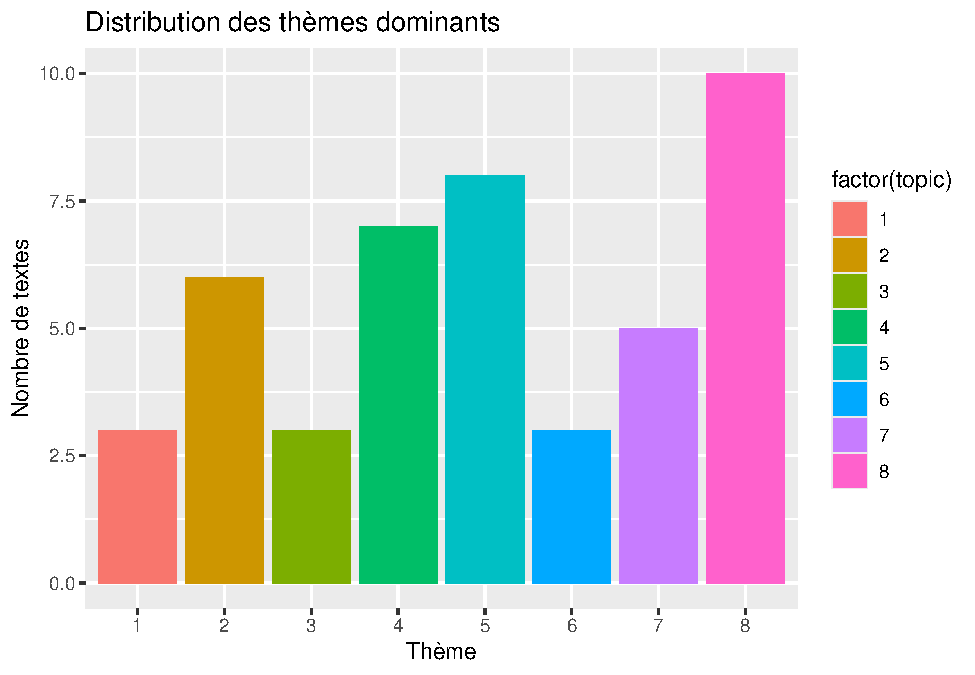
\includegraphics{Texte_mining_files/figure-latex/unnamed-chunk-37-1.pdf}

\subsubsection{Labellisation (très
subjective)}\label{labellisation-truxe8s-subjective}

\begin{Shaded}
\begin{Highlighting}[]
\CommentTok{\# Labelliser les thèmes}

\NormalTok{textes\_gamma }\OtherTok{\textless{}{-}}\NormalTok{ textes\_gamma }\SpecialCharTok{\%\textgreater{}\%}
  \FunctionTok{mutate}\NormalTok{(}\AttributeTok{topic\_label =} \FunctionTok{case\_when}\NormalTok{(}
\NormalTok{    topic }\SpecialCharTok{==} \DecValTok{1} \SpecialCharTok{\textasciitilde{}} \StringTok{"Diversité culturelle et activités communes"}\NormalTok{,}
\NormalTok{    topic }\SpecialCharTok{==} \DecValTok{2} \SpecialCharTok{\textasciitilde{}} \StringTok{"Performances artistiques et intervention scénique"}\NormalTok{,}
\NormalTok{    topic }\SpecialCharTok{==} \DecValTok{3} \SpecialCharTok{\textasciitilde{}} \StringTok{"Présentation des cultures par les communautés"}\NormalTok{,}
\NormalTok{    topic }\SpecialCharTok{==} \DecValTok{4} \SpecialCharTok{\textasciitilde{}} \StringTok{"Aménagement de l\textquotesingle{}espace et la gestion du temps"}\NormalTok{,}
\NormalTok{    topic }\SpecialCharTok{==} \DecValTok{5} \SpecialCharTok{\textasciitilde{}} \StringTok{"Organisation"}\NormalTok{,}
\NormalTok{    topic }\SpecialCharTok{==} \DecValTok{6} \SpecialCharTok{\textasciitilde{}} \StringTok{"Suggestions d\textquotesingle{}amélioration"}\NormalTok{,}
\NormalTok{    topic }\SpecialCharTok{==} \DecValTok{7} \SpecialCharTok{\textasciitilde{}} \StringTok{"Organisation générale et impression globale"}\NormalTok{,}
\NormalTok{    topic }\SpecialCharTok{==} \DecValTok{8} \SpecialCharTok{\textasciitilde{}} \StringTok{"animation"}\NormalTok{,}
    \ConstantTok{TRUE} \SpecialCharTok{\textasciitilde{}} \StringTok{"Autre"}
\NormalTok{  ))}
\end{Highlighting}
\end{Shaded}

\section{4. Approche Alternative avec BERTopic}\label{sec:importation}

BERTopic est un outil puissant de topic modeling (modélisation de
sujets) qui permet d'extraire automatiquement des thèmes principaux à
partir de textes non structurés. Il se distingue des approches
classiques comme LDA par sa capacité à capturer des relations
sémantiques en se basant sur le texte et non des motstokenisés.

\subsection{Installation de miniconda et chargement du package
reticulate}\label{installation-de-miniconda-et-chargement-du-package-reticulate}

Pour utiliser les bibliothèques Python dans R (comme bertopic,
sentence-transformers, etc.) qui sont nécessaire à notre analyse, on
utilise le package reticulate, qui agit comme un pont entre R et Python.
Afin d'assurer que tout fonctionne dans un environnement propre et
contrôlé, nous allons installer Miniconda, une version légère de Conda,
qui sert à gérer les environnements Python.

\begin{Shaded}
\begin{Highlighting}[]
\FunctionTok{library}\NormalTok{(reticulate)}

\CommentTok{\# Voir l\textquotesingle{}environnement actif de reticulate}

\FunctionTok{py\_config}\NormalTok{()}
\end{Highlighting}
\end{Shaded}

\begin{verbatim}
## Error in python_config_impl(python) : 
##   Error 103 occurred running C:/Users/lenovo/Documents/.virtualenvs/r-reticulate/Scripts/python.exe:
\end{verbatim}

\begin{verbatim}
## python:         C:/Users/lenovo/AppData/Local/R/cache/R/reticulate/uv/cache/archive-v0/6h8sIL35_M-JaWAg2n46t/Scripts/python.exe
## libpython:      C:/Users/lenovo/AppData/Local/R/cache/R/reticulate/uv/python/cpython-3.11.12-windows-x86_64-none/python311.dll
## pythonhome:     C:/Users/lenovo/AppData/Local/R/cache/R/reticulate/uv/cache/archive-v0/6h8sIL35_M-JaWAg2n46t
## virtualenv:     C:/Users/lenovo/AppData/Local/R/cache/R/reticulate/uv/cache/archive-v0/6h8sIL35_M-JaWAg2n46t/Scripts/activate_this.py
## version:        3.11.12 (main, Apr  9 2025, 04:03:34) [MSC v.1943 64 bit (AMD64)]
## Architecture:   64bit
## numpy:          C:/Users/lenovo/AppData/Local/R/cache/R/reticulate/uv/cache/archive-v0/6h8sIL35_M-JaWAg2n46t/Lib/site-packages/numpy
## numpy_version:  2.2.4
## 
## NOTE: Python version was forced by py_require()
\end{verbatim}

\begin{Shaded}
\begin{Highlighting}[]
\CommentTok{\# Installation des packages nécessaires dans l’environnement actif de reticulate}
\NormalTok{reticulate}\SpecialCharTok{::}\FunctionTok{py\_install}\NormalTok{(}
  \AttributeTok{packages =} \FunctionTok{c}\NormalTok{(}\StringTok{"sentence{-}transformers"}\NormalTok{, }\StringTok{"hdbscan"}\NormalTok{, }\StringTok{"umap{-}learn"}\NormalTok{, }\StringTok{"bertopic"}\NormalTok{),}
  \AttributeTok{pip =} \ConstantTok{TRUE}
\NormalTok{)}
\end{Highlighting}
\end{Shaded}

\subsubsection{Importation des modules
Python}\label{importation-des-modules-python}

Chaque module que nous importons est lié à une fonctionnalité clé :

\begin{itemize}
\tightlist
\item
  sentence\_transformers : gestion des modèles d'embedding de texte
\item
  hdbscan : algorithme de clustering utilisé par BERTopic
\item
  bertopic : la librairie principale pour la modélisation de sujets
\item
  umap : utilisé pour projeter les embeddings dans un espace de plus
  faible dimension
\end{itemize}

\begin{Shaded}
\begin{Highlighting}[]
\NormalTok{sentence\_transformers }\OtherTok{\textless{}{-}} \FunctionTok{import}\NormalTok{(}\StringTok{"sentence\_transformers"}\NormalTok{)}
\NormalTok{hdbscan }\OtherTok{\textless{}{-}} \FunctionTok{import}\NormalTok{(}\StringTok{"hdbscan"}\NormalTok{)}
\NormalTok{bertopic }\OtherTok{\textless{}{-}} \FunctionTok{import}\NormalTok{(}\StringTok{"bertopic"}\NormalTok{)}
\NormalTok{umap }\OtherTok{\textless{}{-}} \FunctionTok{import}\NormalTok{(}\StringTok{"umap"}\NormalTok{)  }\CommentTok{\# important pour fixer le random\_state}
\end{Highlighting}
\end{Shaded}

\begin{Shaded}
\begin{Highlighting}[]
\CommentTok{\# 🔤 Modèle d\textquotesingle{}embedding (changeable par d\textquotesingle{}autres plus bas)}
\NormalTok{embedding\_model }\OtherTok{\textless{}{-}}\NormalTok{ sentence\_transformers}\SpecialCharTok{$}\FunctionTok{SentenceTransformer}\NormalTok{(}\StringTok{"paraphrase{-}MiniLM{-}L6{-}v2"}\NormalTok{)}
\end{Highlighting}
\end{Shaded}

Ici on utilise `paraphrase-MiniLM-L6-v2', un modèle rapide et efficace.
Mais il existe d'autres variétés plus puissante mais qui sont plus
robuste. Le tableau qui suit donne quelques détails.

\begin{Shaded}
\begin{Highlighting}[]
\CommentTok{\# 🧮 Comparaison de modèles d\textquotesingle{}embedding pour BERTopic}
\NormalTok{embedding\_models }\OtherTok{\textless{}{-}} \FunctionTok{data.frame}\NormalTok{(}
  \AttributeTok{Modele =} \FunctionTok{c}\NormalTok{(}
    \StringTok{"paraphrase{-}distilbert{-}base{-}nli{-}stsb"}\NormalTok{,}
    \StringTok{"bert{-}base{-}nli{-}mean{-}tokens"}\NormalTok{,}
    \StringTok{"all{-}mpnet{-}base{-}v2"}
\NormalTok{  ),}
  \AttributeTok{Taille =} \FunctionTok{c}\NormalTok{(}\DecValTok{768}\NormalTok{, }\DecValTok{768}\NormalTok{, }\DecValTok{768}\NormalTok{),}
  \AttributeTok{Precision\_Semantique =} \FunctionTok{c}\NormalTok{(}
    \StringTok{"Bonne précision sémantique"}\NormalTok{,}
    \StringTok{"Très bonne précision sémantique"}\NormalTok{,}
    \StringTok{"Excellente précision sémantique"}
\NormalTok{  )}
\NormalTok{)}
\CommentTok{\# 📊 Affichage du tableau}
\NormalTok{knitr}\SpecialCharTok{::}\FunctionTok{kable}\NormalTok{(embedding\_models, }\AttributeTok{caption =} \StringTok{"Tableau comparatif de modèles d\textquotesingle{}embedding utilisables avec BERTopic"}\NormalTok{)}
\end{Highlighting}
\end{Shaded}

\begin{longtable}[]{@{}
  >{\raggedright\arraybackslash}p{(\columnwidth - 4\tabcolsep) * \real{0.4800}}
  >{\raggedleft\arraybackslash}p{(\columnwidth - 4\tabcolsep) * \real{0.0933}}
  >{\raggedright\arraybackslash}p{(\columnwidth - 4\tabcolsep) * \real{0.4267}}@{}}
\caption{Tableau comparatif de modèles d'embedding utilisables avec
BERTopic}\tabularnewline
\toprule\noalign{}
\begin{minipage}[b]{\linewidth}\raggedright
Modele
\end{minipage} & \begin{minipage}[b]{\linewidth}\raggedleft
Taille
\end{minipage} & \begin{minipage}[b]{\linewidth}\raggedright
Precision\_Semantique
\end{minipage} \\
\midrule\noalign{}
\endfirsthead
\toprule\noalign{}
\begin{minipage}[b]{\linewidth}\raggedright
Modele
\end{minipage} & \begin{minipage}[b]{\linewidth}\raggedleft
Taille
\end{minipage} & \begin{minipage}[b]{\linewidth}\raggedright
Precision\_Semantique
\end{minipage} \\
\midrule\noalign{}
\endhead
\bottomrule\noalign{}
\endlastfoot
paraphrase-distilbert-base-nli-stsb & 768 & Bonne précision
sémantique \\
bert-base-nli-mean-tokens & 768 & Très bonne précision sémantique \\
all-mpnet-base-v2 & 768 & Excellente précision sémantique \\
\end{longtable}

\begin{Shaded}
\begin{Highlighting}[]
\NormalTok{hdbscan\_model }\OtherTok{\textless{}{-}}\NormalTok{ hdbscan}\SpecialCharTok{$}\FunctionTok{HDBSCAN}\NormalTok{(}
  \AttributeTok{min\_cluster\_size =}\NormalTok{ reticulate}\SpecialCharTok{::}\FunctionTok{r\_to\_py}\NormalTok{(}\DecValTok{3}\DataTypeTok{L}\NormalTok{),}
  \AttributeTok{min\_samples =}\NormalTok{ reticulate}\SpecialCharTok{::}\FunctionTok{r\_to\_py}\NormalTok{(}\DecValTok{1}\DataTypeTok{L}\NormalTok{)}
\NormalTok{)}

\CommentTok{\# 🎯 Réduction de dimension via UMAP avec seed fixée pour reproductibilité}
\NormalTok{umap\_model }\OtherTok{\textless{}{-}}\NormalTok{ umap}\SpecialCharTok{$}\FunctionTok{UMAP}\NormalTok{(}
  \AttributeTok{n\_neighbors =} \DecValTok{15}\DataTypeTok{L}\NormalTok{,}
  \AttributeTok{n\_components =} \DecValTok{5}\DataTypeTok{L}\NormalTok{,}
  \AttributeTok{min\_dist =} \FloatTok{0.0}\NormalTok{,}
  \AttributeTok{metric =} \StringTok{"cosine"}\NormalTok{,}
  \AttributeTok{random\_state =} \DecValTok{42}\DataTypeTok{L}  \CommentTok{\# ✅ Seed fixée ici}
\NormalTok{)}

\CommentTok{\# 📚 Création du modèle BERTopic}
\NormalTok{topic\_model }\OtherTok{\textless{}{-}}\NormalTok{ bertopic}\SpecialCharTok{$}\FunctionTok{BERTopic}\NormalTok{(}
  \AttributeTok{language =} \StringTok{"french"}\NormalTok{,}
  \AttributeTok{embedding\_model =}\NormalTok{ embedding\_model,}
  \AttributeTok{hdbscan\_model =}\NormalTok{ hdbscan\_model,}
  \AttributeTok{umap\_model =}\NormalTok{ umap\_model}
\NormalTok{)}

\CommentTok{\# 📦 Préparation des données}

\NormalTok{docs }\OtherTok{\textless{}{-}}\NormalTok{ Texte\_JI\_filtered}\SpecialCharTok{$}\NormalTok{Texte}
\NormalTok{ids }\OtherTok{\textless{}{-}}\NormalTok{ Texte\_JI\_filtered}\SpecialCharTok{$}\NormalTok{id  }\CommentTok{\# on garde l\textquotesingle{}id associé à chaque texte}

\NormalTok{result }\OtherTok{\textless{}{-}}\NormalTok{ topic\_model}\SpecialCharTok{$}\FunctionTok{fit\_transform}\NormalTok{(docs)}


\CommentTok{\# 🎯 Extraction des résultats}
\NormalTok{topics }\OtherTok{\textless{}{-}}\NormalTok{ result[[}\DecValTok{1}\NormalTok{]]}
\NormalTok{probs }\OtherTok{\textless{}{-}}\NormalTok{ result[[}\DecValTok{2}\NormalTok{]]}

\NormalTok{topics}
\end{Highlighting}
\end{Shaded}

\begin{verbatim}
##  [1] 4 3 5 3 1 0 0 0 2 2 1 0 2 2 3 0 5 0 3 4 1 1 1 1 3 3 1 0 0 2 0 4 0 0 0 0 1 2
## [39] 1 5 4 0 1 0 4
\end{verbatim}

\begin{Shaded}
\begin{Highlighting}[]
\NormalTok{probs}
\end{Highlighting}
\end{Shaded}

\begin{verbatim}
##  [1] 0.7649678 1.0000000 1.0000000 0.7850124 1.0000000 0.8767291 1.0000000
##  [8] 1.0000000 1.0000000 1.0000000 0.9240548 1.0000000 0.8713598 1.0000000
## [15] 1.0000000 1.0000000 1.0000000 0.9533261 1.0000000 1.0000000 1.0000000
## [22] 0.9240548 0.9210614 1.0000000 0.8374228 0.6877206 1.0000000 1.0000000
## [29] 1.0000000 0.8713598 1.0000000 1.0000000 0.9533261 1.0000000 0.8585130
## [36] 1.0000000 1.0000000 0.9615890 0.9210614 1.0000000 1.0000000 1.0000000
## [43] 1.0000000 1.0000000 0.8038874
\end{verbatim}

\begin{Shaded}
\begin{Highlighting}[]
\CommentTok{\# 🔁 Reconstruction du data.frame avec id + texte + classe}
\NormalTok{base\_categorisee }\OtherTok{\textless{}{-}} \FunctionTok{data.frame}\NormalTok{(}
  \AttributeTok{id =}\NormalTok{ ids,}
  \AttributeTok{texte =}\NormalTok{ docs,}
  \AttributeTok{classe =}\NormalTok{ topics,}
  \AttributeTok{proba =}\NormalTok{ probs}
\NormalTok{)}

\CommentTok{\# 🔍 Affichage des infos sur les thèmes trouvés}
\NormalTok{topic\_info }\OtherTok{\textless{}{-}}\NormalTok{ topic\_model}\SpecialCharTok{$}\FunctionTok{get\_topic\_info}\NormalTok{()}
\FunctionTok{head}\NormalTok{(topic\_info)}
\end{Highlighting}
\end{Shaded}

\begin{verbatim}
##   Topic Count                                Name
## 1     0    15                    0_de_la_pays_les
## 2     1    10                1_bien_pour_soit_son
## 3     2     6             2_tout_une_soirée_monde
## 4     3     6        3_sketchs_des_courts_acteurs
## 5     4     5      4_temps_prestations_réduire_le
## 6     5     3 5_court_métrage_culturelle_intégrer
##                                                                                              Representation
## 1                                 de, la, pays, les, présenter, culture, organisation, cultures, chaque, en
## 2                                              bien, pour, soit, son, jours, espace, le, est, journée, tout
## 3                                           tout, une, soirée, monde, voir, salle, grande, dansante, je, un
## 4                                               sketchs, des, courts, acteurs, les, aux, micro, et, je, pas
## 5                               temps, prestations, réduire, le, il, faut, des, chanter, accordez, diminuer
## 6 court, métrage, culturelle, intégrer, créativité, preuve, diversité, participants, sensibiliser, culturel
##                                                                                                                                                                                                                                                                                                                                                                                                                                                                                                                                                                                                                                                 Representative_Docs
## 1 Que chaque pays présente sa culture de telle sorte les personnes qui ne connaissaient pas ce  pays vont le découvrir à travers la prestation de ses résidents, Encourager la co-organisation pour permettre aux différentes cultures de nous présenter des activités culturelles en commun. Prolonger la journée d'intégration à d'autres journées (continuellement) pour favoriser l'apprentissage culturel au sein de l'école, Les différentes communautés doivent s'avantage s'enraciner dans leur cultures et présenter les spécificités de leur cultures afin de susciter la curiousité des autres et voulant en savoir davantage même après la dite journée
## 2                                                                                                                                                                                                                                                                                                                                                                                                                                                       Bien organiser l’événement pour éviter le désordre et les retards., Améliorer le son pour que tout soit bien audible., Vérifier le son pour que tout soit bien clair et qu’on entende bien les prestataires
## 3                                                                                                                                                                                                                                                                                                                                                                                                                        Je ne crois pas qu'on. L'air déjà fait mais je trouve que ça pourrait être intéressant, Utiliser une plus grande salle pour permettre à tout le monde de tout voir, Trouver une salle plus grande pour que tout le monde puisse bien voir.
## 4                                                                                                                                                                                                                                                                                                                              Je suggère des sketchs comiques qui vont nous permettre de réparer les dégâts psychologiques causés par le premier semestre, Faire des sketch courts et donner le micro aux acteurs sur la scène, car habituellement on ne les écoute pas., Faire des sketchs courts et bien donner le micro aux acteurs, qu’on puisse les entendre.
## 5                                                                                                                                                                                                                                                                                                                                                                                                                                                                                                                                                diminuer le temps des discours, Il faut réduire le temps des prestations, Il faut réduire le temps des prestations
## 6                                                                                                                                                                                                                                                                                                                                                                                                                                                                                                                      Faire preuve de créativité, Court métrage culturel, Intégrer un court-métrage sur la diversité culturelle pour sensibiliser les participants
\end{verbatim}

\section{5. Catégorisation}\label{sec:importation}

Dans cette section, nous tentons de catégoriser les textes en se basant
sur les diff'rents thèmes générés par le modèle.

\begin{Shaded}
\begin{Highlighting}[]
\NormalTok{topic\_info}\SpecialCharTok{$}\NormalTok{label }\OtherTok{\textless{}{-}} \FunctionTok{c}\NormalTok{(}
  \StringTok{"Célébration et partage des cultures nationales"}\NormalTok{,               }\CommentTok{\# Topic 0}
  \StringTok{"Aspect technique et organisation"}\NormalTok{,                             }\CommentTok{\# Topic 1}
  \StringTok{"Mieux aménager l\textquotesingle{}espace"}\NormalTok{,                                      }\CommentTok{\# Topic 2}
  \StringTok{"Sketchs et prestations"}\NormalTok{,                                       }\CommentTok{\# Topic 3}
  \StringTok{"Gestion du timing lors des interventions"}\NormalTok{,                     }\CommentTok{\# Topic 4       }
  \StringTok{"Touche créative et courmétrages"}                                  \CommentTok{\# Topic 5}
\NormalTok{)}


\NormalTok{base\_categorisee }\OtherTok{\textless{}{-}} \FunctionTok{merge}\NormalTok{(}
\NormalTok{  base\_categorisee, }
\NormalTok{  topic\_info[, }\FunctionTok{c}\NormalTok{(}\StringTok{"Topic"}\NormalTok{, }\StringTok{"label"}\NormalTok{)], }
  \AttributeTok{by.x =} \StringTok{"classe"}\NormalTok{, }
  \AttributeTok{by.y =} \StringTok{"Topic"}\NormalTok{, }
  \AttributeTok{all.x =} \ConstantTok{TRUE}
\NormalTok{)}


\NormalTok{base\_categorisee }\OtherTok{\textless{}{-}} \FunctionTok{subset}\NormalTok{(base\_categorisee, }\AttributeTok{select =} \SpecialCharTok{{-}}\FunctionTok{c}\NormalTok{(classe, proba))}
\end{Highlighting}
\end{Shaded}

\begin{Shaded}
\begin{Highlighting}[]
\NormalTok{doc\_vides }\OtherTok{\textless{}{-}} \FunctionTok{data.frame}\NormalTok{(}
  \AttributeTok{id =}\NormalTok{ Id\_texte\_NA}
\NormalTok{)}


\CommentTok{\# 2. Identifier les noms des autres colonnes (sauf "document")}
\NormalTok{autres\_colonnes }\OtherTok{\textless{}{-}} \FunctionTok{setdiff}\NormalTok{(}\FunctionTok{names}\NormalTok{(base\_categorisee), }\StringTok{"id"}\NormalTok{)}

\CommentTok{\# 3. Ajouter des NA pour les autres colonnes}
\NormalTok{doc\_vides[autres\_colonnes] }\OtherTok{\textless{}{-}} \ConstantTok{NA}

\CommentTok{\# 4. Fusionner avec la base existante}
\NormalTok{textes\_by\_topic\_complet }\OtherTok{\textless{}{-}} \FunctionTok{rbind}\NormalTok{(base\_categorisee, doc\_vides)}

\CommentTok{\# 5. Optionnel: trier par document si nécessaire}
\NormalTok{textes\_by\_topic\_complet }\OtherTok{\textless{}{-}}\NormalTok{ textes\_by\_topic\_complet[}\FunctionTok{order}\NormalTok{(textes\_by\_topic\_complet}\SpecialCharTok{$}\NormalTok{id), ]}

\CommentTok{\# Joindre les thèmes dominants avec les tweets originaux}

\NormalTok{Texte\_JI}\SpecialCharTok{$}\NormalTok{Texte }\OtherTok{\textless{}{-}} \ConstantTok{NULL}

\NormalTok{textes\_classified }\OtherTok{\textless{}{-}}\NormalTok{ Texte\_JI }\SpecialCharTok{\%\textgreater{}\%}
  \FunctionTok{inner\_join}\NormalTok{(textes\_by\_topic\_complet, }\AttributeTok{by =} \FunctionTok{c}\NormalTok{(}\StringTok{"id"} \OtherTok{=} \StringTok{"id"}\NormalTok{))}

\FunctionTok{head}\NormalTok{(textes\_classified)}
\end{Highlighting}
\end{Shaded}

\begin{verbatim}
## # A tibble: 6 x 5
##      id `Classe de l’étudiant :` `Nationalité de l'étudiant` texte         label
##   <dbl> <chr>                    <chr>                       <chr>         <chr>
## 1     1 AS2                      Congo                       <NA>          <NA> 
## 2     2 ISEP1                    Cameroun                    Donner à tem~ Gest~
## 3     3 AS2                      Congo                       <NA>          <NA> 
## 4     4 AS1                      Sénégal                     Faire des sk~ Sket~
## 5     5 AS1                      Cameroun                    Intégrer un ~ Touc~
## 6     6 ISE1 Eco                 Sénégal                     <NA>          <NA>
\end{verbatim}

\begin{longtable}[]{@{}
  >{\centering\arraybackslash}p{(\columnwidth - 4\tabcolsep) * \real{0.0336}}
  >{\centering\arraybackslash}p{(\columnwidth - 4\tabcolsep) * \real{0.6218}}
  >{\raggedright\arraybackslash}p{(\columnwidth - 4\tabcolsep) * \real{0.3445}}@{}}
\caption{💡 Suggestions pour améliorer l'organisation de la journée
d'intégration}\tabularnewline
\toprule\noalign{}
\begin{minipage}[b]{\linewidth}\centering
id
\end{minipage} & \begin{minipage}[b]{\linewidth}\centering
texte
\end{minipage} & \begin{minipage}[b]{\linewidth}\raggedright
label
\end{minipage} \\
\midrule\noalign{}
\endfirsthead
\toprule\noalign{}
\begin{minipage}[b]{\linewidth}\centering
id
\end{minipage} & \begin{minipage}[b]{\linewidth}\centering
texte
\end{minipage} & \begin{minipage}[b]{\linewidth}\raggedright
label
\end{minipage} \\
\midrule\noalign{}
\endhead
\bottomrule\noalign{}
\endlastfoot
1 & NA & NA \\
2 & Donner à temps le micro aux personnes qui vont chanter. & Gestion du
timing lors des interventions \\
3 & NA & NA \\
4 & Faire des sketchs courts et bien donner le micro aux acteurs. &
Sketchs et prestations \\
5 & Intégrer un court-métrage sur la diversité culturelle pour
sensibiliser. & Touche créative et courmétrages \\
6 & NA & NA \\
7 & Faire des sketch courts et donner le micro aux acteurs sur la scène.
& Sketchs et prestations \\
8 & NA & NA \\
9 & Améliorer le son pour que tout soit bien audible. & Aspect technique
et organisation \\
10 & NA & NA \\
\end{longtable}

\newpage
\section{CONCLUSION}\label{sec:importation}

L'analyse des questions ouvertes à l'aide des techniques de text mining
met en lumière l'importance du \textbf{prétraitement} des données
textuelles. Cette étape cruciale permet de nettoyer, normaliser et
structurer le texte afin de le rendre exploitable pour les algorithmes
d'analyse. Cependant, il est important de noter que les outils de
prétraitement sont plus adaptés et optimisés pour \textbf{l'anglais},
notamment en ce qui concerne les listes de \textbf{stop words}, les
outils de \textbf{stemming} ou de \textbf{lemmatisation}. Cela constitue
un frein lorsqu'on travaille sur des textes en français ou dans d'autres
langues moins représentées.

Parmi les méthodes explorées, \textbf{LDA (Latent Dirichlet Allocation)}
permet d'identifier des thématiques en se basant sur la fréquence des
mots. Toutefois, cette approche présente des \textbf{limites
importantes} : elle repose uniquement sur la \textbf{co-occurrence de
mots}, sans prendre en compte leur sens réel ou leur contexte
sémantique. Ainsi, des textes exprimant des idées similaires avec des
mots différents peuvent ne pas être associés au même thème, ce qui
réduit la pertinence de l'analyse dans certains cas.

C'est dans ce cadre que *BERTopic** se distingue. En s'appuyant sur des
modèles d'embeddings comme BERT, il permet de capter la sémantique des
phrases. Il devient alors possible de regrouper des textes similaires
même si les mots employés sont différents. Cette approche offre une
compréhension plus fine et plus pertinente des idées exprimées dans les
données.

Cela dit, il est essentiel de garder à l'esprit que le traitement des
textes reste une tâche \textbf{complexe} et \textbf{imparfaite}. La
diversité des styles, des formulations, des niveaux de langue ou encore
des erreurs d'écriture rend l'analyse automatique difficile. Les
résultats doivent donc être interprétés avec précaution, et idéalement
complétés par une validation \textbf{humaine} pour garantir leur
fiabilité.

\section{Références
Bibliographiques}\label{ruxe9fuxe9rences-bibliographiques}

\begin{itemize}
\item
  \href{https://www.innovatiana.com/post/best-datasets-for-text-classification}{Classification}
\item
  \href{https://guides.library.upenn.edu/penntdm/r}{Prétraitement}
\item
  \href{https://bookdown.org/tianyuan09/ai4ph2022/tutorial.html}{Prétraitement}
\item
  \href{https://ladal.edu.au/tutorials/topic/topic.html?}{Topic
  modeling}
\end{itemize}

\end{document}
